%&preformat-present

\newif\ifpresentation % Условие, проверяющее, что документ --- презентация
\presentationtrue
\documentclass[10pt, xcolor={dvipsnames, table, hyperref}]{beamer}

%%%%%%%%%%%%%%%%%%%%%%%%%%%%%%%%%%%%%%%%%%%%%%%%%%%%%%%
%%%% Файл упрощённых настроек шаблона автореферата %%%%
%%%%%%%%%%%%%%%%%%%%%%%%%%%%%%%%%%%%%%%%%%%%%%%%%%%%%%%

%%% Инициализирование переменных, не трогать!  %%%
\newcounter{showperssign}
\newcounter{showsecrsign}
\newcounter{showopplead}
%%%%%%%%%%%%%%%%%%%%%%%%%%%%%%%%%%%%%%%%%%%%%%%%%%%%%%%

%%% Список публикаций %%%
\makeatletter
\@ifundefined{c@usefootcite}{
  \newcounter{usefootcite}
  \setcounter{usefootcite}{0} % 0 --- два списка литературы;
                              % 1 --- список публикаций автора + цитирование
                              %       других работ в сносках
}{}
\makeatother

\makeatletter
\@ifundefined{c@bibgrouped}{
  \newcounter{bibgrouped}
  \setcounter{bibgrouped}{0}  % 0 --- единый список работ автора;
                              % 1 --- сгруппированные работы автора
}{}
\makeatother

%%% Область упрощённого управления оформлением %%%

%% Управление зазором между подрисуночной подписью и основным текстом %%
\setlength{\belowcaptionskip}{10pt plus 20pt minus 2pt}


%% Подпись таблиц %%

% смещение строк подписи после первой
\newcommand{\tabindent}{0cm}

% тип форматирования таблицы
% plain --- название и текст в одной строке
% split --- название и текст в разных строках
\newcommand{\tabformat}{plain}

%%% настройки форматирования таблицы `plain'

% выравнивание по центру подписи, состоящей из одной строки
% true  --- выравнивать
% false --- не выравнивать
\newcommand{\tabsinglecenter}{false}

% выравнивание подписи таблиц
% justified   --- выравнивать как обычный текст
% centering   --- выравнивать по центру
% centerlast  --- выравнивать по центру только последнюю строку
% centerfirst --- выравнивать по центру только первую строку
% raggedleft  --- выравнивать по правому краю
% raggedright --- выравнивать по левому краю
\newcommand{\tabjust}{justified}

% Разделитель записи «Таблица #» и названия таблицы
\newcommand{\tablabelsep}{~\cyrdash\ }

%%% настройки форматирования таблицы `split'

% положение названия таблицы
% \centering   --- выравнивать по центру
% \raggedleft  --- выравнивать по правому краю
% \raggedright --- выравнивать по левому краю
\newcommand{\splitformatlabel}{\raggedleft}

% положение текста подписи
% \centering   --- выравнивать по центру
% \raggedleft  --- выравнивать по правому краю
% \raggedright --- выравнивать по левому краю
\newcommand{\splitformattext}{\raggedright}

%% Подпись рисунков %%
%Разделитель записи «Рисунок #» и названия рисунка
\newcommand{\figlabelsep}{~\cyrdash\ }  % (ГОСТ 2.105, 4.3.1)
                                        % "--- здесь не работает

%Демонстрация подписи диссертанта на автореферате
\setcounter{showperssign}{1}  % 0 --- не показывать;
                              % 1 --- показывать
%Демонстрация подписи учёного секретаря на автореферате
\setcounter{showsecrsign}{1}  % 0 --- не показывать;
                              % 1 --- показывать
%Демонстрация информации об оппонентах и ведущей организации на автореферате
\setcounter{showopplead}{1}   % 0 --- не показывать;
                              % 1 --- показывать

%%% Цвета гиперссылок %%%
% Latex color definitions: http://latexcolor.com/
\definecolor{linkcolor}{rgb}{0.9,0,0}
\definecolor{citecolor}{rgb}{0,0.6,0}
\definecolor{urlcolor}{rgb}{0,0,1}
%\definecolor{linkcolor}{rgb}{0,0,0} %black
%\definecolor{citecolor}{rgb}{0,0,0} %black
%\definecolor{urlcolor}{rgb}{0,0,0} %black               % Общие настройки шаблона
%%% Проверка используемого TeX-движка %%%
\newif\ifxetexorluatex   % определяем новый условный оператор (http://tex.stackexchange.com/a/47579)
\ifxetex
    \xetexorluatextrue
\else
    \ifluatex
        \xetexorluatextrue
    \else
        \xetexorluatexfalse
    \fi
\fi

\newif\ifsynopsis           % Условие, проверяющее, что документ --- автореферат

\usepackage{etoolbox}[2015/08/02]   % Для продвинутой проверки разных условий
\providebool{presentation}

\usepackage{comment}    % Позволяет убирать блоки текста (добавляет
                        % окружение comment и команду \excludecomment)

%%% Поля и разметка страницы %%%
\usepackage{pdflscape}  % Для включения альбомных страниц
\usepackage{geometry}   % Для последующего задания полей

%%% Математические пакеты %%%
\usepackage{amsthm,amsmath,amscd}   % Математические дополнения от AMS
\usepackage{amsfonts,amssymb}       % Математические дополнения от AMS
\usepackage{mathtools}              % Добавляет окружение multlined
\usepackage{xfrac}                  % Красивые дроби
\usepackage[
    locale = DE,
    list-separator       = {;\,},
    list-final-separator = {;\,},
    list-pair-separator  = {;\,},
    list-units           = single,
    range-units          = single,
    range-phrase={\text{\ensuremath{-}}},
    % quotient-mode        = fraction, % красивые дроби могут не соответствовать ГОСТ
    fraction-function    = \sfrac,
    separate-uncertainty,
    ]{siunitx}                      % Размерности SI
\sisetup{inter-unit-product = \ensuremath{{}\cdot{}}}

% Кириллица в нумерации subequations
% Для правильной работы требуется выполнение сразу после загрузки пакетов
\patchcmd{\subequations}{\def\theequation{\theparentequation\alph{equation}}}
{\def\theequation{\theparentequation\asbuk{equation}}}
{\typeout{subequations patched}}{\typeout{subequations not patched}}

%%%% Установки для размера шрифта 14 pt %%%%
%% Формирование переменных и констант для сравнения (один раз для всех подключаемых файлов)%%
%% должно располагаться до вызова пакета fontspec или polyglossia, потому что они сбивают его работу
\newlength{\curtextsize}
\newlength{\bigtextsize}
\setlength{\bigtextsize}{13.9pt}

\makeatletter
%\show\f@size    % неплохо для отслеживания, но вызывает стопорение процесса,
                 % если документ компилируется без команды  -interaction=nonstopmode
\setlength{\curtextsize}{\f@size pt}
\makeatother

%%% Кодировки и шрифты %%%
\ifxetexorluatex
    \ifpresentation
        \providecommand*\autodot{} % quick fix for polyglossia 1.50
    \fi
    \PassOptionsToPackage{no-math}{fontspec}    % https://tex.stackexchange.com/a/26295/104425
    \usepackage{polyglossia}[2014/05/21]        % Поддержка многоязычности
                                        % (fontspec подгружается автоматически)
\else
   %%% Решение проблемы копирования текста в буфер кракозябрами
    \ifnumequal{\value{usealtfont}}{0}{}{
        \input glyphtounicode.tex
        \input glyphtounicode-cmr.tex %from pdfx package
        \pdfgentounicode=1
    }
    \usepackage{cmap}   % Улучшенный поиск русских слов в полученном pdf-файле
    \ifnumequal{\value{usealtfont}}{2}{}{
        \defaulthyphenchar=127  % Если стоит до fontenc, то переносы
                                % не впишутся в выделяемый текст при
                                % копировании его в буфер обмена
    }
    \usepackage{textcomp}
    \usepackage[T1,T2A]{fontenc}                    % Поддержка русских букв
    \ifnumequal{\value{usealtfont}}{1}{% Используется pscyr, при наличии
        \IfFileExists{pscyr.sty}{\usepackage{pscyr}}{}  % Подключение pscyr
    }{}
    \usepackage[utf8]{inputenc}[2014/04/30]         % Кодировка utf8
    \usepackage[english, russian]{babel}[2014/03/24]% Языки: русский, английский
    \makeatletter\AtBeginDocument{\let\@elt\relax}\makeatother % babel 3.40 fix
    \ifnumequal{\value{usealtfont}}{2}{
        % http://dxdy.ru/post1238763.html#p1238763
        \usepackage[scaled=0.914]{XCharter}[2017/12/19] % Подключение русифицированных шрифтов XCharter
        \usepackage[charter, vvarbb, scaled=1.048]{newtxmath}[2017/12/14]
        \ifpresentation
        \else
            \setDisplayskipStretch{-0.078}
        \fi
    }{}
\fi

%%% Оформление абзацев %%%
\ifpresentation
\else
    \indentafterchapter     % Красная строка после заголовков типа chapter
    \usepackage{indentfirst}
\fi

%%% Цвета %%%
\ifpresentation
\else
    \usepackage[dvipsnames, table, hyperref]{xcolor} % Совместимо с tikz
\fi

%%% Таблицы %%%
\usepackage{longtable,ltcaption} % Длинные таблицы
\usepackage{multirow,makecell}   % Улучшенное форматирование таблиц
\usepackage{tabu, tabulary}      % таблицы с автоматически подбирающейся
                                 % шириной столбцов (tabu обязательно
                                 % до hyperref вызывать)
\usepackage{threeparttable}      % автоматический подгон ширины подписи таблицы

%%% Общее форматирование
\usepackage{soulutf8}% Поддержка переносоустойчивых подчёркиваний и зачёркиваний
\usepackage{icomma}  % Запятая в десятичных дробях

%%% Оптимизация расстановки переносов и длины последней строки абзаца
\IfFileExists{impnattypo.sty}{% проверка установленности пакета impnattypo
    \ifluatex
        \ifnumequal{\value{draft}}{1}{% Черновик
            \usepackage[hyphenation, lastparline, nosingleletter, homeoarchy,
            rivers, draft]{impnattypo}
        }{% Чистовик
            \usepackage[hyphenation, lastparline, nosingleletter]{impnattypo}
        }
    \else
        \usepackage[hyphenation, lastparline]{impnattypo}
    \fi
}{}

%% Векторная графика

\usepackage{tikz}                   % Продвинутый пакет векторной графики
\usetikzlibrary{chains}             % Для примера tikz рисунка
\usetikzlibrary{shapes.geometric}   % Для примера tikz рисунка
\usetikzlibrary{shapes.symbols}     % Для примера tikz рисунка
\usetikzlibrary{arrows}             % Для примера tikz рисунка

%%% Гиперссылки %%%
\ifxetexorluatex
    \let\CYRDZE\relax
\fi
\usepackage{hyperref}[2012/11/06]

%%% Изображения %%%
\usepackage{graphicx}[2014/04/25]   % Подключаем пакет работы с графикой
\usepackage{caption}                % Подписи рисунков и таблиц
\usepackage{subcaption}             % Подписи подрисунков и подтаблиц
\usepackage{pdfpages}               % Добавление внешних pdf файлов

%%% Счётчики %%%
\usepackage{aliascnt}
\usepackage[figure,table]{totalcount}   % Счётчик рисунков и таблиц
\usepackage{totcount}   % Пакет создания счётчиков на основе последнего номера
                        % подсчитываемого элемента (может требовать дважды
                        % компилировать документ)
\usepackage{totpages}   % Счётчик страниц, совместимый с hyperref (ссылается
                        % на номер последней страницы). Желательно ставить
                        % последним пакетом в преамбуле

%%% Продвинутое управление групповыми ссылками (пока только формулами) %%%
\ifpresentation
\else
    \usepackage[russian]{cleveref} % cleveref имеет сложности со считыванием
    % языка из babel. Такое решение русификации вывода выбрано вместо
    % определения в documentclass из опасности что-то лишнее передать во все
    % остальные пакеты, включая библиографию.

    % Добавление возможности использования пробелов в \labelcref
    % https://tex.stackexchange.com/a/340502/104425
    \usepackage{kvsetkeys}
    \makeatletter
    \let\org@@cref\@cref
    \renewcommand*{\@cref}[2]{%
        \edef\process@me{%
            \noexpand\org@@cref{#1}{\zap@space#2 \@empty}%
        }\process@me
    }
    \makeatother
\fi

\usepackage{placeins} % для \FloatBarrier


% sorokin
\usepackage{amsmath}


\ifnumequal{\value{draft}}{1}{% Черновик
    \usepackage[firstpage]{draftwatermark}
    \SetWatermarkText{DRAFT}
    \SetWatermarkFontSize{14pt}
    \SetWatermarkScale{15}
    \SetWatermarkAngle{45}
}{}

%%% Цитата, не приводимая в автореферате:
% возможно, актуальна только для biblatex
%\newcommand{\citeinsynopsis}[1]{\ifsynopsis\else ~\cite{#1} \fi}

% если текущий процесс запущен библиотекой tikz-external, то прекомпиляция должна быть включена
\ifdefined\tikzexternalrealjob
    \setcounter{imgprecompile}{1}
\fi

\ifnumequal{\value{imgprecompile}}{1}{% Только если у нас включена предкомпиляция
    \usetikzlibrary{external}   % подключение возможности предкомпиляции
    \tikzexternalize[prefix=images/cache/,optimize command away=\includepdf] % activate! % здесь можно указать отдельную папку для скомпилированных файлов
    \ifxetex
        \tikzset{external/up to date check={diff}}
    \fi
}{}
            % Пакеты общие для диссертации и автореферата
%%% Основные сведения %%%
\newcommand{\thesisAuthorLastName}{Сорокин}
\newcommand{\thesisAuthorOtherNames}{Дитрий Игоревич}
\newcommand{\thesisAuthorInitials}{\fixme{Д.\,И.}}
\newcommand{\thesisAuthor}             % Диссертация, ФИО автора
{%
    \texorpdfstring{% \texorpdfstring takes two arguments and uses the first for (La)TeX and the second for pdf
        \thesisAuthorLastName~\thesisAuthorOtherNames% так будет отображаться на титульном листе или в тексте, где будет использоваться переменная
    }{%
        \thesisAuthorLastName, \thesisAuthorOtherNames% эта запись для свойств pdf-файла. В таком виде, если pdf будет обработан программами для сбора библиографических сведений, будет правильно представлена фамилия.
    }
}
\newcommand{\thesisAuthorShort}        % Диссертация, ФИО автора инициалами
{\thesisAuthorInitials~\thesisAuthorLastName}
%\newcommand{\thesisUdk}                % Диссертация, УДК
%{\fixme{xxx.xxx}}
\newcommand{\thesisTitle}              % Диссертация, название
{
Применение машинного обучения с подкреплением для управления робототехническими устройствами и виртуальными агентами}
\newcommand{\thesisSpecialtyNumber}    % Диссертация, специальность, номер
{05.13.18}
\newcommand{\thesisSpecialtyTitle}     % Диссертация, специальность, название (название взято с сайта ВАК для примера)
{Математическое моделирование, численные методы и комплексы программ}
%% \newcommand{\thesisSpecialtyTwoNumber} % Диссертация, вторая специальность, номер
%% {\fixme{XX.XX.XX}}
%% \newcommand{\thesisSpecialtyTwoTitle}  % Диссертация, вторая специальность, название
%% {\fixme{Теория и~методика физического воспитания, спортивной тренировки,
%% оздоровительной и~адаптивной физической культуры}}
\newcommand{\thesisDegree}             % Диссертация, ученая степень
{кандидата технических наук}
\newcommand{\thesisDegreeShort}        % Диссертация, ученая степень, краткая запись
{\fixme{канд. физ.-мат. наук}}
\newcommand{\thesisCity}               % Диссертация, город написания диссертации
{Мсква}
\newcommand{\thesisYear}               % Диссертация, год написания диссертации
{\the\year}
\newcommand{\thesisOrganization}       % Диссертация, организация
{Федеральное государственное автономное образовательное учреждение высшего образования <<Московский физико-технический институт (национальный исследовательский университет)>> <<МФТИ>>}
\newcommand{\thesisOrganizationShort}  % Диссертация, краткое название организации для доклада
{\fixme{НазУчДисРаб}}

\newcommand{\thesisInOrganization}     % Диссертация, организация в предложном падеже: Работа выполнена в ...
{\fixme{учреждении с~длинным длинным длинным длинным названием, в~котором
выполнялась данная диссертационная работа}}

%% \newcommand{\supervisorDead}{}           % Рисовать рамку вокруг фамилии
\newcommand{\supervisorFio}              % Научный руководитель, ФИО
{Львовский Александр Исаевич}
\newcommand{\supervisorRegalia}          % Научный руководитель, регалии
{кандидат физико-математических наук, профессор}
\newcommand{\supervisorFioShort}         % Научный руководитель, ФИО
{\fixme{И.\,О.~Фамилия}}
\newcommand{\supervisorRegaliaShort}     % Научный руководитель, регалии
{\fixme{уч.~ст.,~уч.~зв.}}

%% \newcommand{\supervisorTwoDead}{}        % Рисовать рамку вокруг фамилии
%% \newcommand{\supervisorTwoFio}           % Второй научный руководитель, ФИО
%% {\fixme{Фамилия Имя Отчество}}
%% \newcommand{\supervisorTwoRegalia}       % Второй научный руководитель, регалии
%% {\fixme{уч. степень, уч. звание}}
%% \newcommand{\supervisorTwoFioShort}      % Второй научный руководитель, ФИО
%% {\fixme{И.\,О.~Фамилия}}
%% \newcommand{\supervisorTwoRegaliaShort}  % Второй научный руководитель, регалии
%% {\fixme{уч.~ст.,~уч.~зв.}}

\newcommand{\opponentOneFio}           % Оппонент 1, ФИО
{\fixme{Фамилия Имя Отчество}}
\newcommand{\opponentOneRegalia}       % Оппонент 1, регалии
{\fixme{доктор физико-математических наук, профессор}}
\newcommand{\opponentOneJobPlace}      % Оппонент 1, место работы
{\fixme{Не очень длинное название для места работы}}
\newcommand{\opponentOneJobPost}       % Оппонент 1, должность
{\fixme{старший научный сотрудник}}

\newcommand{\opponentTwoFio}           % Оппонент 2, ФИО
{\fixme{Фамилия Имя Отчество}}
\newcommand{\opponentTwoRegalia}       % Оппонент 2, регалии
{\fixme{кандидат физико-математических наук}}
\newcommand{\opponentTwoJobPlace}      % Оппонент 2, место работы
{\fixme{Основное место работы c длинным длинным длинным длинным названием}}
\newcommand{\opponentTwoJobPost}       % Оппонент 2, должность
{\fixme{старший научный сотрудник}}

%% \newcommand{\opponentThreeFio}         % Оппонент 3, ФИО
%% {\fixme{Фамилия Имя Отчество}}
%% \newcommand{\opponentThreeRegalia}     % Оппонент 3, регалии
%% {\fixme{кандидат физико-математических наук}}
%% \newcommand{\opponentThreeJobPlace}    % Оппонент 3, место работы
%% {\fixme{Основное место работы c длинным длинным длинным длинным названием}}
%% \newcommand{\opponentThreeJobPost}     % Оппонент 3, должность
%% {\fixme{старший научный сотрудник}}

\newcommand{\leadingOrganizationTitle} % Ведущая организация, дополнительные строки. Удалить, чтобы не отображать в автореферате
{\fixme{Федеральное государственное бюджетное образовательное учреждение высшего
профессионального образования с~длинным длинным длинным длинным названием}}

\newcommand{\defenseDate}              % Защита, дата
{\fixme{DD mmmmmmmm YYYY~г.~в~XX часов}}
\newcommand{\defenseCouncilNumber}     % Защита, номер диссертационного совета
{\fixme{Д\,123.456.78}}
\newcommand{\defenseCouncilTitle}      % Защита, учреждение диссертационного совета
{\fixme{Название учреждения}}
\newcommand{\defenseCouncilAddress}    % Защита, адрес учреждение диссертационного совета
{\fixme{Адрес}}
\newcommand{\defenseCouncilPhone}      % Телефон для справок
{\fixme{+7~(0000)~00-00-00}}

\newcommand{\defenseSecretaryFio}      % Секретарь диссертационного совета, ФИО
{\fixme{Фамилия Имя Отчество}}
\newcommand{\defenseSecretaryRegalia}  % Секретарь диссертационного совета, регалии
{\fixme{д-р~физ.-мат. наук}}            % Для сокращений есть ГОСТы, например: ГОСТ Р 7.0.12-2011 + http://base.garant.ru/179724/#block_30000

\newcommand{\synopsisLibrary}          % Автореферат, название библиотеки
{\fixme{Название библиотеки}}
\newcommand{\synopsisDate}             % Автореферат, дата рассылки
{\fixme{DD mmmmmmmm}\the\year~года}

% To avoid conflict with beamer class use \providecommand
\providecommand{\keywords}%            % Ключевые слова для метаданных PDF диссертации и автореферата
{}
                % Основные сведения
\input{common/fonts}               % Определение шрифтов (частичное)

%%%%%%%%%%%%%%%%%%%%%%%%%%%%%%%%%%%%%%%%%%%%%%%%%%%%%%%
%%%% Файл упрощённых настроек шаблона автореферата %%%%
%%%%%%%%%%%%%%%%%%%%%%%%%%%%%%%%%%%%%%%%%%%%%%%%%%%%%%%

%%% Инициализирование переменных, не трогать!  %%%
\newcounter{showperssign}
\newcounter{showsecrsign}
\newcounter{showopplead}
%%%%%%%%%%%%%%%%%%%%%%%%%%%%%%%%%%%%%%%%%%%%%%%%%%%%%%%

%%% Список публикаций %%%
\makeatletter
\@ifundefined{c@usefootcite}{
  \newcounter{usefootcite}
  \setcounter{usefootcite}{0} % 0 --- два списка литературы;
                              % 1 --- список публикаций автора + цитирование
                              %       других работ в сносках
}{}
\makeatother

\makeatletter
\@ifundefined{c@bibgrouped}{
  \newcounter{bibgrouped}
  \setcounter{bibgrouped}{0}  % 0 --- единый список работ автора;
                              % 1 --- сгруппированные работы автора
}{}
\makeatother

%%% Область упрощённого управления оформлением %%%

%% Управление зазором между подрисуночной подписью и основным текстом %%
\setlength{\belowcaptionskip}{10pt plus 20pt minus 2pt}


%% Подпись таблиц %%

% смещение строк подписи после первой
\newcommand{\tabindent}{0cm}

% тип форматирования таблицы
% plain --- название и текст в одной строке
% split --- название и текст в разных строках
\newcommand{\tabformat}{plain}

%%% настройки форматирования таблицы `plain'

% выравнивание по центру подписи, состоящей из одной строки
% true  --- выравнивать
% false --- не выравнивать
\newcommand{\tabsinglecenter}{false}

% выравнивание подписи таблиц
% justified   --- выравнивать как обычный текст
% centering   --- выравнивать по центру
% centerlast  --- выравнивать по центру только последнюю строку
% centerfirst --- выравнивать по центру только первую строку
% raggedleft  --- выравнивать по правому краю
% raggedright --- выравнивать по левому краю
\newcommand{\tabjust}{justified}

% Разделитель записи «Таблица #» и названия таблицы
\newcommand{\tablabelsep}{~\cyrdash\ }

%%% настройки форматирования таблицы `split'

% положение названия таблицы
% \centering   --- выравнивать по центру
% \raggedleft  --- выравнивать по правому краю
% \raggedright --- выравнивать по левому краю
\newcommand{\splitformatlabel}{\raggedleft}

% положение текста подписи
% \centering   --- выравнивать по центру
% \raggedleft  --- выравнивать по правому краю
% \raggedright --- выравнивать по левому краю
\newcommand{\splitformattext}{\raggedright}

%% Подпись рисунков %%
%Разделитель записи «Рисунок #» и названия рисунка
\newcommand{\figlabelsep}{~\cyrdash\ }  % (ГОСТ 2.105, 4.3.1)
                                        % "--- здесь не работает

%Демонстрация подписи диссертанта на автореферате
\setcounter{showperssign}{1}  % 0 --- не показывать;
                              % 1 --- показывать
%Демонстрация подписи учёного секретаря на автореферате
\setcounter{showsecrsign}{1}  % 0 --- не показывать;
                              % 1 --- показывать
%Демонстрация информации об оппонентах и ведущей организации на автореферате
\setcounter{showopplead}{1}   % 0 --- не показывать;
                              % 1 --- показывать

%%% Цвета гиперссылок %%%
% Latex color definitions: http://latexcolor.com/
\definecolor{linkcolor}{rgb}{0.9,0,0}
\definecolor{citecolor}{rgb}{0,0.6,0}
\definecolor{urlcolor}{rgb}{0,0,1}
%\definecolor{linkcolor}{rgb}{0,0,0} %black
%\definecolor{citecolor}{rgb}{0,0,0} %black
%\definecolor{urlcolor}{rgb}{0,0,0} %black         % Настройки презентации
\hypersetup{
    unicode=true,          % non-Latin characters in Acrobat’s bookmarks
}
\usepackage{mathtext}
\usepackage{enumerate,float,indentfirst}
\usepackage{appendixnumberbeamer} % не считать номера страниц после команды \appendix
\usepackage{array, booktabs} % для таблиц
\usepackage{pgfpages}
\usepackage{esint} % various fancy integral symbols
\usepackage{media9} % dsorokin
\usepackage{algorithm2e} %dsorokin
%\usepackage{enumitem} %dsorokin
\usepackage{algpseudocode} %dsorokin
\usepackage{ifthen} %dsorokin
\usepackage{dirtytalk} %dsorokin

\graphicspath{{images/}{Presentation/images/}} % папки с графикой

\DeclareRobustCommand{\fixme}{\textcolor{red}}       % решаем проблему превращения названия цвета в результате \MakeUppercase, http://tex.stackexchange.com/a/187930, \DeclareRobustCommand protects \todo from expanding inside \MakeUppercase

\makeatletter
\newcommand*{\rom}[1]{\expandafter\@slowromancap\romannumeral#1@}
\makeatother

\newcommand{\itemi}{\item[\checkmark]}

\algnewcommand\algorithmicforeach{\textbf{for each}}
\algdef{S}[FOR]{ForEach}[1]{\algorithmicforeach\ #1\ \algorithmicdo}

\let\origfootnotemark\footnotemark
\renewcommand{\footnotemark}[1][]{%
    \ifthenelse{\equal{#1}{}}{%
        \origfootnotemark%
    }{%
        \def\nextitem{\def\nextitem{\textsuperscript{,}}}% Separator
        \renewcommand*{\do}[1]{\nextitem\origfootnotemark[##1]}% How to process each item
        \docsvlist{#1}% Process list
    }%
}  % Библиотеки презентации
% Общие стили оформления.
% Возможные варианты значений ищите в описании библиотеки beamer
%\usetheme{Pittsburgh}
%\usecolortheme{whale}

\usetheme[progressbar=foot]{metropolis}
\setbeamertemplate{caption*}[numbered]

% \usetheme[secheader]{Boadilla}
% \usecolortheme{seahorse}

% Размер полей слайдов
\setbeamersize{text margin left=1cm,%
               text margin right=1cm}

% выключение кнопок навигации
\beamertemplatenavigationsymbolsempty

% Размеры шрифтов
\setbeamerfont{title}{size=\large}
\setbeamerfont{subtitle}{size=\small}
\setbeamerfont{author}{size=\normalsize}
\setbeamerfont{institute}{size=\small}
\setbeamerfont{date}{size=\normalsize}
\setbeamerfont{bibliography item}{size=\small}
\setbeamerfont{bibliography entry author}{size=\small}
\setbeamerfont{bibliography entry title}{size=\small}
\setbeamerfont{bibliography entry location}{size=\small}
\setbeamerfont{bibliography entry note}{size=\small}
% Аналогично можно настроить и другие размеры.
% Названия классов элементов можно найти здесь
% http://www.cpt.univ-mrs.fr/~masson/latex/Beamer-appearance-cheat-sheet.pdf

% Цвет элементов
%\setbeamercolor{footline}{fg=blue}
%\setbeamercolor{bibliography item}{fg=black}
%\setbeamercolor{bibliography entry author}{fg=black}
%\setbeamercolor{bibliography entry title}{fg=black}
%\setbeamercolor{bibliography entry location}{fg=black}
%\setbeamercolor{bibliography entry note}{fg=black}
% Аналогично можно настроить и другие цвета.
% Названия классов элементов можно найти здесь
% http://www.cpt.univ-mrs.fr/~masson/latex/Beamer-appearance-cheat-sheet.pdf

% Нумеровать список статей
% https://tex.stackexchange.com/a/419506/104425
\setbeamertemplate{bibliography item}{\insertbiblabel}
% или убрать номера
% \setbeamertemplate{bibliography item}{}

% Использовать шрифт с засечками для формул
% https://tex.stackexchange.com/a/34267/104425
\usefonttheme[onlymath]{serif}

% https://tex.stackexchange.com/a/291545/104425
\makeatletter
\def\beamer@framenotesbegin{% at beginning of slide
    \usebeamercolor[fg]{normal text}
    \gdef\beamer@noteitems{}%
    \gdef\beamer@notes{}%
}
\makeatother

% footer презентации
\setbeamertemplate{footline}{
    \leavevmode%
    \hbox{%
        \begin{beamercolorbox}[wd=.333333\paperwidth,ht=2.25ex,dp=1ex,center]{}%
            % И. О. Фамилия, Организация кратко
            \thesisAuthorShort, \thesisOrganizationShort
        \end{beamercolorbox}%
        \begin{beamercolorbox}[wd=.333333\paperwidth,ht=2.25ex,dp=1ex,center]{}%
            % Город, 20XX
            \thesisCity, \thesisYear
        \end{beamercolorbox}%
        \begin{beamercolorbox}[wd=.333333\paperwidth,ht=2.25ex,dp=1ex,right]{}%
            Стр. \insertframenumber{} из \inserttotalframenumber \hspace*{2ex}
        \end{beamercolorbox}}%
    \vskip0pt%
}

% вывод на экран заметок к презентации
\ifnumequal{\value{presnotes}}{0}{}{
    \setbeameroption{show notes}
    \ifnumequal{\value{presnotes}}{2}{
        \setbeameroption{show notes on second screen=\presposition}
    }{}
}
        % Стили презентации
\iffalse
\setbeamertemplate{title page}
{
    \ifnumequal{\value{logotitle}}{1}{
        \IfFileExists{images/logo.pdf}{
            \begin{minipage}[c]{0.15\textwidth}
                \begin{flushleft}
                    \usebeamercolor[fg]{titlegraphic}\inserttitlegraphic
                \end{flushleft}
            \end{minipage}%
            \hfill
            \begin{minipage}[c]{0.8\linewidth}
                \centering
                \usebeamerfont{institute}\insertinstitute\par
            \end{minipage}
        }{
            \centering
            \usebeamerfont{institute}\insertinstitute\par
        }
    }{
        \centering
        \usebeamerfont{institute}\insertinstitute\par
    }
    \centering
    \vfill
    \usebeamerfont{subtitle}\insertsubtitle\par
    \bigskip
    \usebeamerfont{title}\inserttitle\par
    \vfill
    \usebeamerfont{author}\insertauthor\par
    \vfill
    \usebeamerfont{date}\insertdate\par
}
\fi

%\title{\small{Название презентации}}
\title{\thesisTitle}
\author{%
    \texorpdfstring{%
        \emph{Выступающий:}~\thesisAuthorShort\\%
        \emph{Руководитель:}~\supervisorRegaliaShort~\supervisorFioShort\\%
        %
    }{\thesisAuthor}%
}

\subtitle{Представление на соискание учёной степени \thesisDegree\ }
%по специальности \thesisSpecialtyNumber\ \thesisSpecialtyTitle}

\date{\vspace{60pt} \centering \texorpdfstring{\thesisCity, \thesisYear}{}}
         % Настройки заглавной странице

% Новые переменные, которые могут использоваться во всём проекте
% ГОСТ 7.0.11-2011
% 9.2 Оформление текста автореферата диссертации
% 9.2.1 Общая характеристика работы включает в себя следующие основные структурные
% элементы:
% актуальность темы исследования;
\newcommand{\actualityTXT}{Актуальность темы.}
% степень ее разработанности;
\newcommand{\progressTXT}{Степень разработанности темы.}
% цели и задачи;
\newcommand{\aimTXT}{Целью}
\newcommand{\tasksTXT}{задачи}
% научную новизну;
\newcommand{\noveltyTXT}{Научная новизна:}
% теоретическую и практическую значимость работы;
%\newcommand{\influenceTXT}{Теоретическая и практическая значимость}
% или чаще используют просто
\newcommand{\influenceTXT}{Практическая значимость}
% методологию и методы исследования;
\newcommand{\methodsTXT}{Методология и методы исследования.}
% положения, выносимые на защиту;
\newcommand{\defpositionsTXT}{Основные положения, выносимые на~защиту:}
% степень достоверности и апробацию результатов.
\newcommand{\reliabilityTXT}{Достоверность}
\newcommand{\probationTXT}{Апробация работы.}

\newcommand{\contributionTXT}{Личный вклад.}
\newcommand{\publicationsTXT}{Публикации.}


%%% Заголовки библиографии:

% для автореферата:
\newcommand{\bibtitleauthor}{Публикации автора по теме диссертации}

% для стиля библиографии `\insertbiblioauthorgrouped`
\newcommand{\bibtitleauthorvak}{В изданиях из списка ВАК РФ}
\newcommand{\bibtitleauthorscopus}{В изданиях, входящих в международную базу цитирования Scopus}
\newcommand{\bibtitleauthorwos}{В изданиях, входящих в международную базу цитирования Web of Science}
\newcommand{\bibtitleauthorother}{В прочих изданиях}
\newcommand{\bibtitleauthorconf}{В сборниках трудов конференций}
\newcommand{\bibtitleauthorpatent}{Зарегистрированные патенты}
\newcommand{\bibtitleauthorprogram}{Зарегистрированные программы для ЭВМ}

% для стиля библиографии `\insertbiblioauthorimportant`:
\newcommand{\bibtitleauthorimportant}{Наиболее значимые \protect\MakeLowercase\bibtitleauthor}

% для списка литературы в диссертации и списка чужих работ в автореферате:
\newcommand{\bibtitlefull}{Список литературы} % (ГОСТ Р 7.0.11-2011, 4)

% dsorokin
\newcommand{\ex}{\mathop{\mathbb{E}}}

 % dsorokin

%%% Библиография. Выбор движка для реализации %%%
\ifnumequal{\value{bibliosel}}{0}{%
    \input{biblio/predefined}   % Встроенная реализация с загрузкой файла через движок bibtex8
}{
    %%% Реализация библиографии пакетами biblatex и biblatex-gost с использованием движка biber %%%

\usepackage{csquotes} % biblatex рекомендует его подключать. Пакет для оформления сложных блоков цитирования.
%%% Загрузка пакета с основными настройками %%%
\makeatletter
\ifnumequal{\value{draft}}{0}{% Чистовик
\usepackage[%
backend=biber,% движок
bibencoding=utf8,% кодировка bib файла
sorting=none,% настройка сортировки списка литературы
style=gost-numeric,% стиль цитирования и библиографии (по ГОСТ)
language=autobib,% получение языка из babel/polyglossia, default: autobib % если ставить autocite или auto, то цитаты в тексте с указанием страницы, получат указание страницы на языке оригинала
autolang=other,% многоязычная библиография
clearlang=true,% внутренний сброс поля language, если он совпадает с языком из babel/polyglossia
defernumbers=true,% нумерация проставляется после двух компиляций, зато позволяет выцеплять библиографию по ключевым словам и нумеровать не из большего списка
sortcites=true,% сортировать номера затекстовых ссылок при цитировании (если в квадратных скобках несколько ссылок, то отображаться будут отсортированно, а не абы как)
doi=false,% Показывать или нет ссылки на DOI
isbn=false,% Показывать или нет ISBN, ISSN, ISRN
]{biblatex}[2016/09/17]
\ltx@iffilelater{biblatex-gost.def}{2017/05/03}%
{\toggletrue{bbx:gostbibliography}%
\renewcommand*{\revsdnamepunct}{\addcomma}}{}
}{%Черновик
\usepackage[%
backend=biber,% движок
bibencoding=utf8,% кодировка bib файла
sorting=none,% настройка сортировки списка литературы
% defernumbers=true, % откомментируйте, если требуется правильная нумерация ссылок на литературу в режиме черновика. Замедляет сборку
]{biblatex}[2016/09/17]%
}
\makeatother

\providebool{blxmc} % biblatex version needs and has MakeCapital workaround
\boolfalse{blxmc} % setting our new boolean flag to default false
\ifxetexorluatex
\else
% Исправление случая неподдержки знака номера в pdflatex
    \DefineBibliographyStrings{russian}{number={\textnumero}}

% Исправление случая отсутствия прописных букв в некоторых случаях
% https://github.com/plk/biblatex/issues/960#issuecomment-596658282
    \ifdefmacro{\ExplSyntaxOn}{}{\usepackage{expl3}}
    \makeatletter
    \ltx@ifpackagelater{biblatex}{2020/02/23}{
    % Assuming this version of biblatex defines MakeCapital correctly
    }{
        \ltx@ifpackagelater{biblatex}{2019/12/01}{
            % Assuming this version of biblatex defines MakeCapital incorrectly
            \usepackage{expl3}[2020/02/25]
            \@ifpackagelater{expl3}{2020/02/25}{
                \booltrue{blxmc} % setting our new boolean flag to true
            }{}
        }{}
    }
    \makeatother
    \ifblxmc
        \typeout{Assuming this version of biblatex defines MakeCapital
        incorrectly}
        \usepackage{xparse}
        \makeatletter
        \ExplSyntaxOn
        \NewDocumentCommand \blx@maketext@lowercase {m}
          {
            \text_lowercase:n {#1}
          }

        \NewDocumentCommand \blx@maketext@uppercase {m}
          {
            \text_uppercase:n {#1}
          }

        \RenewDocumentCommand \MakeCapital {m}
          {
            \text_titlecase_first:n {#1}
          }
        \ExplSyntaxOff

        \protected\def\blx@biblcstring#1#2#3{%
          \blx@begunit
          \blx@hyphenreset
          \blx@bibstringsimple
          \lowercase{\edef\blx@tempa{#3}}%
          \ifcsundef{#2@\blx@tempa}
            {\blx@warn@nostring\blx@tempa
             \blx@endnounit}
            {#1{\blx@maketext@lowercase{\csuse{#2@\blx@tempa}}}%
             \blx@endunit}}

        \protected\def\blx@bibucstring#1#2#3{%
          \blx@begunit
          \blx@hyphenreset
          \blx@bibstringsimple
          \lowercase{\edef\blx@tempa{#3}}%
          \ifcsundef{#2@\blx@tempa}
            {\blx@warn@nostring\blx@tempa
             \blx@endnounit}
            {#1{\blx@maketext@uppercase{\csuse{#2@\blx@tempa}}}%
             \blx@endunit}}
        \makeatother
    \fi
\fi

\ifsynopsis
\ifnumgreater{\value{usefootcite}}{0}{
    \ExecuteBibliographyOptions{autocite=footnote}
    \newbibmacro*{cite:full}{%
        \printtext[bibhypertarget]{%
            \usedriver{%
                \DeclareNameAlias{sortname}{default}%
            }{%
                \thefield{entrytype}%
            }%
        }%
        \usebibmacro{shorthandintro}%
    }
    \DeclareCiteCommand{\smartcite}[\mkbibfootnote]{%
        \usebibmacro{prenote}%
    }{%
        \usebibmacro{citeindex}%
        \usebibmacro{cite:full}%
    }{%
        \multicitedelim%
    }{%
        \usebibmacro{postnote}%
    }
}{}
\fi

%%% Подключение файлов bib %%%
\addbibresource[label=bl-external]{biblio/external.bib}
\addbibresource[label=bl-author]{biblio/author.bib}
\addbibresource[label=bl-registered]{biblio/registered.bib}

%http://tex.stackexchange.com/a/141831/79756
%There is a way to automatically map the language field to the langid field. The following lines in the preamble should be enough to do that.
%This command will copy the language field into the langid field and will then delete the contents of the language field. The language field will only be deleted if it was successfully copied into the langid field.
\DeclareSourcemap{ %модификация bib файла перед тем, как им займётся biblatex
    \maps{
        \map{% перекидываем значения полей language в поля langid, которыми пользуется biblatex
            \step[fieldsource=language, fieldset=langid, origfieldval, final]
            \step[fieldset=language, null]
        }
        \map{% перекидываем значения полей numpages в поля pagetotal, которыми пользуется biblatex
            \step[fieldsource=numpages, fieldset=pagetotal, origfieldval, final]
            \step[fieldset=numpages, null]
        }
        \map{% перекидываем значения полей pagestotal в поля pagetotal, которыми пользуется biblatex
            \step[fieldsource=pagestotal, fieldset=pagetotal, origfieldval, final]
            \step[fieldset=pagestotal, null]
        }
        \map[overwrite]{% перекидываем значения полей shortjournal, если они есть, в поля journal, которыми пользуется biblatex
            \step[fieldsource=shortjournal, final]
            \step[fieldset=journal, origfieldval]
            \step[fieldset=shortjournal, null]
        }
        \map[overwrite]{% перекидываем значения полей shortbooktitle, если они есть, в поля booktitle, которыми пользуется biblatex
            \step[fieldsource=shortbooktitle, final]
            \step[fieldset=booktitle, origfieldval]
            \step[fieldset=shortbooktitle, null]
        }
        \map{% если в поле medium написано "Электронный ресурс", то устанавливаем поле media, которым пользуется biblatex, в значение eresource.
            \step[fieldsource=medium,
            match=\regexp{Электронный\s+ресурс},
            final]
            \step[fieldset=media, fieldvalue=eresource]
            \step[fieldset=medium, null]
        }
        \map[overwrite]{% стираем значения всех полей issn
            \step[fieldset=issn, null]
        }
        \map[overwrite]{% стираем значения всех полей abstract, поскольку ими не пользуемся, а там бывают "неприятные" латеху символы
            \step[fieldsource=abstract]
            \step[fieldset=abstract,null]
        }
        \map[overwrite]{ % переделка формата записи даты
            \step[fieldsource=urldate,
            match=\regexp{([0-9]{2})\.([0-9]{2})\.([0-9]{4})},
            replace={$3-$2-$1$4}, % $4 вставлен исключительно ради нормальной работы программ подсветки синтаксиса, которые некорректно обрабатывают $ в таких конструкциях
            final]
        }
        \map[overwrite]{ % стираем ключевые слова
            \step[fieldsource=keywords]
            \step[fieldset=keywords,null]
        }
        % реализация foreach различается для biblatex v3.12 и v3.13.
        % Для версии v3.13 эта конструкция заменяет последующие 7 структур map
        % \map[overwrite,foreach={authorvak,authorscopus,authorwos,authorconf,authorother,authorparent,authorprogram}]{ % записываем информацию о типе публикации в ключевые слова
        %     \step[fieldsource=$MAPLOOP,final=true]
        %     \step[fieldset=keywords,fieldvalue={,biblio$MAPLOOP},append=true]
        % }
        \map[overwrite]{ % записываем информацию о типе публикации в ключевые слова
            \step[fieldsource=authorvak,final=true]
            \step[fieldset=keywords,fieldvalue={,biblioauthorvak},append=true]
        }
        \map[overwrite]{ % записываем информацию о типе публикации в ключевые слова
            \step[fieldsource=authorscopus,final=true]
            \step[fieldset=keywords,fieldvalue={,biblioauthorscopus},append=true]
        }
        \map[overwrite]{ % записываем информацию о типе публикации в ключевые слова
            \step[fieldsource=authorwos,final=true]
            \step[fieldset=keywords,fieldvalue={,biblioauthorwos},append=true]
        }
        \map[overwrite]{ % записываем информацию о типе публикации в ключевые слова
            \step[fieldsource=authorconf,final=true]
            \step[fieldset=keywords,fieldvalue={,biblioauthorconf},append=true]
        }
        \map[overwrite]{ % записываем информацию о типе публикации в ключевые слова
            \step[fieldsource=authorother,final=true]
            \step[fieldset=keywords,fieldvalue={,biblioauthorother},append=true]
        }
        \map[overwrite]{ % записываем информацию о типе публикации в ключевые слова
            \step[fieldsource=authorpatent,final=true]
            \step[fieldset=keywords,fieldvalue={,biblioauthorpatent},append=true]
        }
        \map[overwrite]{ % записываем информацию о типе публикации в ключевые слова
            \step[fieldsource=authorprogram,final=true]
            \step[fieldset=keywords,fieldvalue={,biblioauthorprogram},append=true]
        }
        \map[overwrite]{ % добавляем ключевые слова, чтобы различать источники
            \perdatasource{biblio/external.bib}
            \step[fieldset=keywords, fieldvalue={,biblioexternal},append=true]
        }
        \map[overwrite]{ % добавляем ключевые слова, чтобы различать источники
            \perdatasource{biblio/author.bib}
            \step[fieldset=keywords, fieldvalue={,biblioauthor},append=true]
        }
        \map[overwrite]{ % добавляем ключевые слова, чтобы различать источники
            \perdatasource{biblio/registered.bib}
            \step[fieldset=keywords, fieldvalue={,biblioregistered},append=true]
        }
        \map[overwrite]{ % добавляем ключевые слова, чтобы различать источники
            \step[fieldset=keywords, fieldvalue={,bibliofull},append=true]
        }
%        \map[overwrite]{% стираем значения всех полей series
%            \step[fieldset=series, null]
%        }
        \map[overwrite]{% перекидываем значения полей howpublished в поля organization для типа online
            \step[typesource=online, typetarget=online, final]
            \step[fieldsource=howpublished, fieldset=organization, origfieldval]
            \step[fieldset=howpublished, null]
        }
    }
}

\ifnumequal{\value{mediadisplay}}{1}{
    \DeclareSourcemap{
        \maps{%
            \map{% использование media=text по умолчанию
                \step[fieldset=media, fieldvalue=text]
            }
        }
    }
}{}
\ifnumequal{\value{mediadisplay}}{2}{
    \DeclareSourcemap{
        \maps{%
            \map[overwrite]{% удаление всех записей media
                \step[fieldset=media, null]
            }
        }
    }
}{}
\ifnumequal{\value{mediadisplay}}{3}{
    \DeclareSourcemap{
        \maps{
            \map[overwrite]{% стираем значения всех полей media=text
                \step[fieldsource=media,match={text},final]
                \step[fieldset=media, null]
            }
        }
    }
}{}
\ifnumequal{\value{mediadisplay}}{4}{
    \DeclareSourcemap{
        \maps{
            \map[overwrite]{% стираем значения всех полей media=eresource
                \step[fieldsource=media,match={eresource},final]
                \step[fieldset=media, null]
            }
        }
    }
}{}

\ifsynopsis
\else
\DeclareSourcemap{ %модификация bib файла перед тем, как им займётся biblatex
    \maps{
        \map[overwrite]{% стираем значения всех полей addendum
            \perdatasource{biblio/author.bib}
            \step[fieldset=addendum, null] %чтобы избавиться от информации об объёме авторских статей, в отличие от автореферата
        }
    }
}
\fi

%\ifresume
% dsorokin: print quantile of papers 
\DeclareSourcemap{
    \maps[datatype=bibtex]{
      \map{
        \step[fieldsource=quantile]
        \step[fieldset=usera,origfieldval]
    }
  }
}

\DeclareFieldFormat{usera}{(\textbf{#1})}

\AtEveryBibitem{%
    \csappto{blx@bbx@\thefield{entrytype}}{% put at end of entry
        \iffieldundef{usera}{%
        }{%
          \space\printfield{usera}
        }
    }
}

%\fi

\ifpresentation
% удаляем лишние поля в списке литературы презентации
% их названия можно узнать в файле presentation.bbl
\DeclareSourcemap{
    \maps{
    \map[overwrite,foreach={%
        % {{{ Список лишних полей в презентации
        address,%
        chapter,%
        edition,%
        editor,%
        eid,%
        howpublished,%
        institution,%
        key,%
        month,%
        note,%
        number,%
        organization,%
        pages,%
        publisher,%
        school,%
        series,%
        type,%
        media,%
        url,%
        doi,%
        location,%
        volume,%
        % Список лишних полей в презентации }}}
    }]{
        \perdatasource{biblio/author.bib}
        \step[fieldset=$MAPLOOP,null]
    }
    }
}
\fi

\defbibfilter{vakscopuswos}{%
    keyword=biblioauthorvak or keyword=biblioauthorscopus or keyword=biblioauthorwos
}

\defbibfilter{scopuswos}{%
    keyword=biblioauthorscopus or keyword=biblioauthorwos
}

\defbibfilter{papersregistered}{%
    keyword=biblioauthor or keyword=biblioregistered
}

%%% Убираем неразрывные пробелы перед двоеточием и точкой с запятой %%%
%\makeatletter
%\ifnumequal{\value{draft}}{0}{% Чистовик
%    \renewcommand*{\addcolondelim}{%
%      \begingroup%
%      \def\abx@colon{%
%        \ifdim\lastkern>\z@\unkern\fi%
%        \abx@puncthook{:}\space}%
%      \addcolon%
%      \endgroup}
%
%    \renewcommand*{\addsemicolondelim}{%
%      \begingroup%
%      \def\abx@semicolon{%
%        \ifdim\lastkern>\z@\unkern\fi%
%        \abx@puncthook{;}\space}%
%      \addsemicolon%
%      \endgroup}
%}{}
%\makeatother

%%% Правка записей типа thesis, чтобы дважды не писался автор
%\ifnumequal{\value{draft}}{0}{% Чистовик
%\DeclareBibliographyDriver{thesis}{%
%  \usebibmacro{bibindex}%
%  \usebibmacro{begentry}%
%  \usebibmacro{heading}%
%  \newunit
%  \usebibmacro{author}%
%  \setunit*{\labelnamepunct}%
%  \usebibmacro{thesistitle}%
%  \setunit{\respdelim}%
%  %\printnames[last-first:full]{author}%Вот эту строчку нужно убрать, чтобы автор диссертации не дублировался
%  \newunit\newblock
%  \printlist[semicolondelim]{specdata}%
%  \newunit
%  \usebibmacro{institution+location+date}%
%  \newunit\newblock
%  \usebibmacro{chapter+pages}%
%  \newunit
%  \printfield{pagetotal}%
%  \newunit\newblock
%  \usebibmacro{doi+eprint+url+note}%
%  \newunit\newblock
%  \usebibmacro{addendum+pubstate}%
%  \setunit{\bibpagerefpunct}\newblock
%  \usebibmacro{pageref}%
%  \newunit\newblock
%  \usebibmacro{related:init}%
%  \usebibmacro{related}%
%  \usebibmacro{finentry}}
%}{}

%\newbibmacro{string+doi}[1]{% новая макрокоманда на простановку ссылки на doi
%    \iffieldundef{doi}{#1}{\href{http://dx.doi.org/\thefield{doi}}{#1}}}

%\ifnumequal{\value{draft}}{0}{% Чистовик
%\renewcommand*{\mkgostheading}[1]{\usebibmacro{string+doi}{#1}} % ссылка на doi с авторов. стоящих впереди записи
%\renewcommand*{\mkgostheading}[1]{#1} % только лишь убираем курсив с авторов
%}{}
%\DeclareFieldFormat{title}{\usebibmacro{string+doi}{#1}} % ссылка на doi с названия работы
%\DeclareFieldFormat{journaltitle}{\usebibmacro{string+doi}{#1}} % ссылка на doi с названия журнала
%%% Тире как разделитель в библиографии традиционной руской длины:
\renewcommand*{\newblockpunct}{\addperiod\addnbspace\cyrdash\space\bibsentence}
%%% Убрать тире из разделителей элементов в библиографии:
%\renewcommand*{\newblockpunct}{%
%    \addperiod\space\bibsentence}%block punct.,\bibsentence is for vol,etc.
%%% Изменение точки с запятой на запятую в перечислении библиографических
%%% ссылок:
%\renewcommand*{\multicitedelim}{\addcomma\space}

%%% Возвращаем запись «Режим доступа» %%%
%\DefineBibliographyStrings{english}{%
%    urlfrom = {Mode of access}
%}
%\DeclareFieldFormat{url}{\bibstring{urlfrom}\addcolon\space\url{#1}}

%%% В списке литературы обозначение одной буквой диапазона страниц англоязычного источника %%%
\DefineBibliographyStrings{english}{%
    pages = {p\adddot} %заглавность буквы затем по месту определяется работой самого biblatex
}

%%% В ссылке на источник в основном тексте с указанием конкретной страницы обозначение одной большой буквой %%%
%\DefineBibliographyStrings{russian}{%
%    page = {C\adddot}
%}

%%% Исправление длины тире в диапазонах %%%
% \cyrdash --- тире «русской» длины, \textendash --- en-dash
\DefineBibliographyExtras{russian}{%
  \protected\def\bibrangedash{%
    \cyrdash\penalty\value{abbrvpenalty}}% almost unbreakable dash
  \protected\def\bibdaterangesep{\bibrangedash}%тире для дат
}
\DefineBibliographyExtras{english}{%
  \protected\def\bibrangedash{%
    \cyrdash\penalty\value{abbrvpenalty}}% almost unbreakable dash
  \protected\def\bibdaterangesep{\bibrangedash}%тире для дат
}

%Set higher penalty for breaking in number, dates and pages ranges
\setcounter{abbrvpenalty}{10000} % default is \hyphenpenalty which is 12

%Set higher penalty for breaking in names
\setcounter{highnamepenalty}{10000} % If you prefer the traditional BibTeX behavior (no linebreaks at highnamepenalty breakpoints), set it to ‘infinite’ (10 000 or higher).
\setcounter{lownamepenalty}{10000}

%%% Set low penalties for breaks at uppercase letters and lowercase letters
%\setcounter{biburllcpenalty}{500} %управляет разрывами ссылок после маленьких букв RTFM biburllcpenalty
%\setcounter{biburlucpenalty}{3000} %управляет разрывами ссылок после больших букв, RTFM biburlucpenalty

%%% Список литературы с красной строки (без висячего отступа) %%%
%\defbibenvironment{bibliography} % переопределяем окружение библиографии из gost-numeric.bbx пакета biblatex-gost
%  {\list
%     {\printtext[labelnumberwidth]{%
%       \printfield{prefixnumber}%
%       \printfield{labelnumber}}}
%     {%
%      \setlength{\labelwidth}{\labelnumberwidth}%
%      \setlength{\leftmargin}{0pt}% default is \labelwidth
%      \setlength{\labelsep}{\widthof{\ }}% Управляет длиной отступа после точки % default is \biblabelsep
%      \setlength{\itemsep}{\bibitemsep}% Управление дополнительным вертикальным разрывом между записями. \bibitemsep по умолчанию соответствует \itemsep списков в документе.
%      \setlength{\itemindent}{\bibhang}% Пользуемся тем, что \bibhang по умолчанию принимает значение \parindent (абзацного отступа), который переназначен в styles.tex
%      \addtolength{\itemindent}{\labelwidth}% Сдвигаем правее на величину номера с точкой
%      \addtolength{\itemindent}{\labelsep}% Сдвигаем ещё правее на отступ после точки
%      \setlength{\parsep}{\bibparsep}%
%     }%
%      \renewcommand*{\makelabel}[1]{\hss##1}%
%  }
%  {\endlist}
%  {\item}

%%% Макросы автоматического подсчёта количества авторских публикаций.
% Печатают невидимую (пустую) библиографию, считая количество источников.
% http://tex.stackexchange.com/a/66851/79756
%
\makeatletter
    \newtotcounter{citenum}
    \defbibenvironment{counter}
        {\setcounter{citenum}{0}\renewcommand{\blx@driver}[1]{}} % begin code: убирает весь выводимый текст
        {} % end code
        {\stepcounter{citenum}} % item code: cчитает "печатаемые в библиографию" источники

    \newtotcounter{citeauthorvak}
    \defbibenvironment{countauthorvak}
        {\setcounter{citeauthorvak}{0}\renewcommand{\blx@driver}[1]{}}
        {}
        {\stepcounter{citeauthorvak}}

    \newtotcounter{citeauthorscopus}
    \defbibenvironment{countauthorscopus}
        {\setcounter{citeauthorscopus}{0}\renewcommand{\blx@driver}[1]{}}
        {}
        {\stepcounter{citeauthorscopus}}

    \newtotcounter{citeauthorwos}
    \defbibenvironment{countauthorwos}
        {\setcounter{citeauthorwos}{0}\renewcommand{\blx@driver}[1]{}}
        {}
        {\stepcounter{citeauthorwos}}

    \newtotcounter{citeauthorother}
    \defbibenvironment{countauthorother}
        {\setcounter{citeauthorother}{0}\renewcommand{\blx@driver}[1]{}}
        {}
        {\stepcounter{citeauthorother}}

    \newtotcounter{citeauthorconf}
    \defbibenvironment{countauthorconf}
        {\setcounter{citeauthorconf}{0}\renewcommand{\blx@driver}[1]{}}
        {}
        {\stepcounter{citeauthorconf}}

    \newtotcounter{citeauthor}
    \defbibenvironment{countauthor}
        {\setcounter{citeauthor}{0}\renewcommand{\blx@driver}[1]{}}
        {}
        {\stepcounter{citeauthor}}

    \newtotcounter{citeauthorvakscopuswos}
    \defbibenvironment{countauthorvakscopuswos}
        {\setcounter{citeauthorvakscopuswos}{0}\renewcommand{\blx@driver}[1]{}}
        {}
        {\stepcounter{citeauthorvakscopuswos}}

    \newtotcounter{citeauthorscopuswos}
    \defbibenvironment{countauthorscopuswos}
        {\setcounter{citeauthorscopuswos}{0}\renewcommand{\blx@driver}[1]{}}
        {}
        {\stepcounter{citeauthorscopuswos}}

    \newtotcounter{citeregistered}
    \defbibenvironment{countregistered}
        {\setcounter{citeregistered}{0}\renewcommand{\blx@driver}[1]{}}
        {}
        {\stepcounter{citeregistered}}

    \newtotcounter{citeauthorpatent}
    \defbibenvironment{countauthorpatent}
        {\setcounter{citeauthorpatent}{0}\renewcommand{\blx@driver}[1]{}}
        {}
        {\stepcounter{citeauthorpatent}}

    \newtotcounter{citeauthorprogram}
    \defbibenvironment{countauthorprogram}
        {\setcounter{citeauthorprogram}{0}\renewcommand{\blx@driver}[1]{}}
        {}
        {\stepcounter{citeauthorprogram}}

    \newtotcounter{citeexternal}
    \defbibenvironment{countexternal}
        {\setcounter{citeexternal}{0}\renewcommand{\blx@driver}[1]{}}
        {}
        {\stepcounter{citeexternal}}
\makeatother

\defbibheading{nobibheading}{} % пустой заголовок, для подсчёта публикаций с помощью невидимой библиографии
\defbibheading{pubgroup}{\section*{#1}} % обычный стиль, заголовок-секция
\defbibheading{pubsubgroup}{\noindent\textbf{#1}} % для подразделов "по типу источника"

%%%Сортировка списка литературы Русский-Английский (предварительно удалить dissertation.bbl) (начало)
%%%Источник: https://github.com/odomanov/biblatex-gost/wiki/%D0%9A%D0%B0%D0%BA-%D1%81%D0%B4%D0%B5%D0%BB%D0%B0%D1%82%D1%8C,-%D1%87%D1%82%D0%BE%D0%B1%D1%8B-%D1%80%D1%83%D1%81%D1%81%D0%BA%D0%BE%D1%8F%D0%B7%D1%8B%D1%87%D0%BD%D1%8B%D0%B5-%D0%B8%D1%81%D1%82%D0%BE%D1%87%D0%BD%D0%B8%D0%BA%D0%B8-%D0%BF%D1%80%D0%B5%D0%B4%D1%88%D0%B5%D1%81%D1%82%D0%B2%D0%BE%D0%B2%D0%B0%D0%BB%D0%B8-%D0%BE%D1%81%D1%82%D0%B0%D0%BB%D1%8C%D0%BD%D1%8B%D0%BC
%\DeclareSourcemap{
%    \maps[datatype=bibtex]{
%        \map{
%            \step[fieldset=langid, fieldvalue={tempruorder}]
%        }
%        \map[overwrite]{
%            \step[fieldsource=langid, match=russian, final]
%            \step[fieldsource=presort,
%            match=\regexp{(.+)},
%            replace=\regexp{aa$1}]
%        }
%        \map{
%            \step[fieldsource=langid, match=russian, final]
%            \step[fieldset=presort, fieldvalue={az}]
%        }
%        \map[overwrite]{
%            \step[fieldsource=langid, notmatch=russian, final]
%            \step[fieldsource=presort,
%            match=\regexp{(.+)},
%            replace=\regexp{za$1}]
%        }
%        \map{
%            \step[fieldsource=langid, notmatch=russian, final]
%            \step[fieldset=presort, fieldvalue={zz}]
%        }
%        \map{
%            \step[fieldsource=langid, match={tempruorder}, final]
%            \step[fieldset=langid, null]
%        }
%    }
%}
%Сортировка списка литературы (конец)

%%% Создание команд для вывода списка литературы %%%
\newcommand*{\insertbibliofull}{
    \printbibliography[keyword=bibliofull,section=0,title=\bibtitlefull]
    \ifnumequal{\value{draft}}{0}{
      \printbibliography[heading=nobibheading,env=counter,keyword=bibliofull,section=0]
    }{}
}
\newcommand*{\insertbiblioauthor}{
    \printbibliography[heading=pubgroup, section=0, filter=papersregistered, title=\bibtitleauthor]
}
\newcommand*{\insertbiblioauthorimportant}{
    \printbibliography[heading=pubgroup, section=2, filter=papersregistered, title=\bibtitleauthorimportant]
}

% Вариант вывода печатных работ автора, с группировкой по типу источника.
% Порядок команд `\printbibliography` должен соответствовать порядку в файле common/characteristic.tex
\newcommand*{\insertbiblioauthorgrouped}{
    \section*{\bibtitleauthor}
    \ifsynopsis
    \printbibliography[heading=pubsubgroup, section=0, keyword=biblioauthorvak,    title=\bibtitleauthorvak,resetnumbers=true] % Работы автора из списка ВАК (сброс нумерации)
    \else
    \printbibliography[heading=pubsubgroup, section=0, keyword=biblioauthorvak,    title=\bibtitleauthorvak,resetnumbers=false] % Работы автора из списка ВАК (сквозная нумерация)
    \fi
    \printbibliography[heading=pubsubgroup, section=0, keyword=biblioauthorwos,    title=\bibtitleauthorwos,resetnumbers=false]% Работы автора, индексируемые Web of Science
    \printbibliography[heading=pubsubgroup, section=0, keyword=biblioauthorscopus, title=\bibtitleauthorscopus,resetnumbers=false]% Работы автора, индексируемые Scopus
    \printbibliography[heading=pubsubgroup, section=0, keyword=biblioauthorpatent, title=\bibtitleauthorpatent,resetnumbers=false]% Патенты
    \printbibliography[heading=pubsubgroup, section=0, keyword=biblioauthorprogram,title=\bibtitleauthorprogram,resetnumbers=false]% Программы для ЭВМ
    \printbibliography[heading=pubsubgroup, section=0, keyword=biblioauthorconf,   title=\bibtitleauthorconf,resetnumbers=false]% Тезисы конференций
    \printbibliography[heading=pubsubgroup, section=0, keyword=biblioauthorother,  title=\bibtitleauthorother,resetnumbers=false]% Прочие работы автора
}

\newcommand*{\insertbiblioexternal}{
    \printbibliography[heading=pubgroup,    section=0, keyword=biblioexternal,     title=\bibtitlefull]
}
     % Реализация пакетом biblatex через движок biber
}

% Вывести информацию о версиях используемых библиотек в лог сборки
\listfiles

\begin{document}
\begin{frame}[noframenumbering,plain]
    \setcounter{framenumber}{1}
    \maketitle
\end{frame}

\begin{frame}
\frametitle{Обучение с подкреплением}
\begin{columns}
\column{0.4\linewidth}
  \centering
    \begin{tikzpicture}
            \node[anchor=south west,inner sep=0] (image) at (0,0) {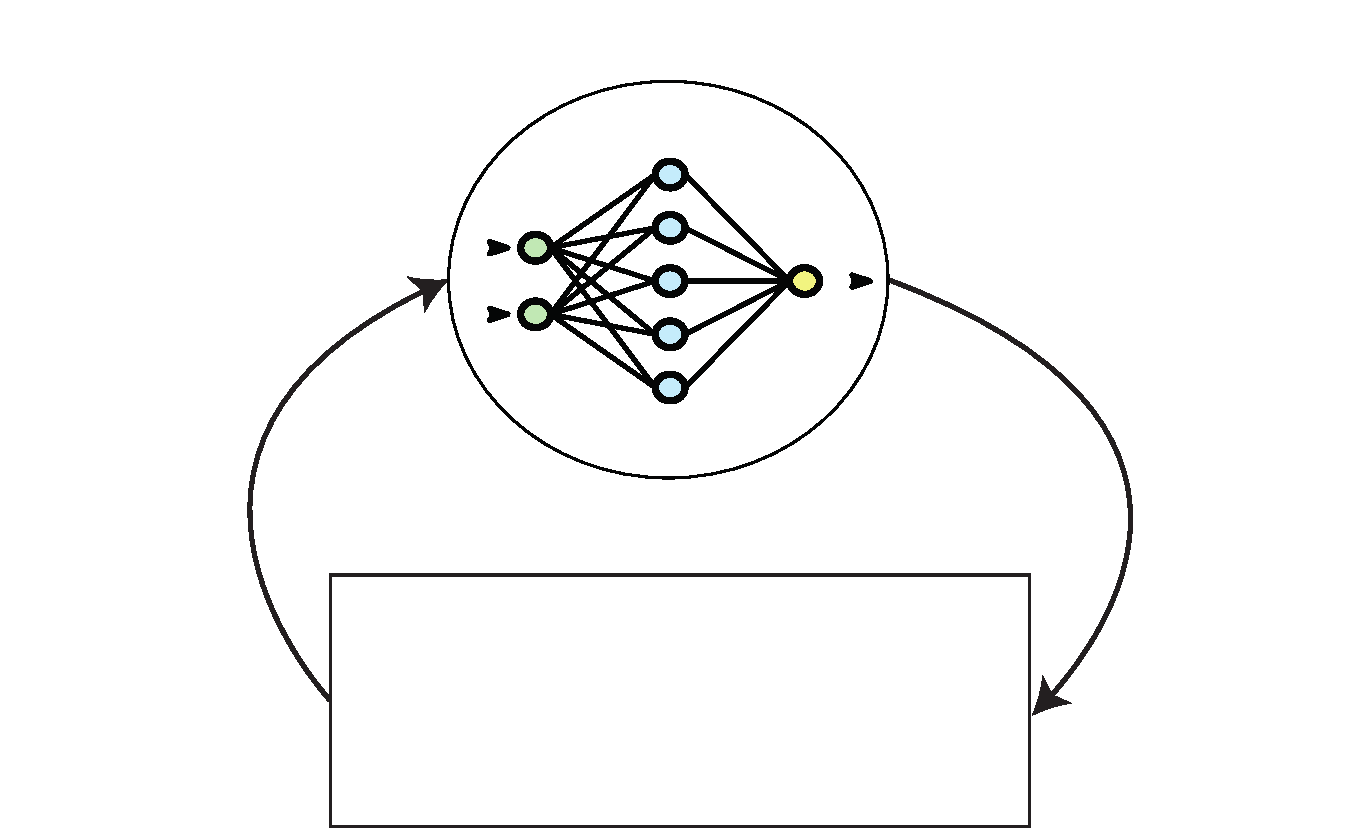
\includegraphics[width=1\linewidth]{Presentation/images/rl_setting_no_text.pdf}};
            \node[align=center,font={\small}] at (0.4,1) {s, r,\\done};
            \node[align=center,font={\small}] at (2.2,0.4) {среда};
            \node[align=center,font={\small}] at (2.1,2.6) {агент};
            \node[align=center,font={\small}] at (3.8,1) {a};
        \end{tikzpicture}
  %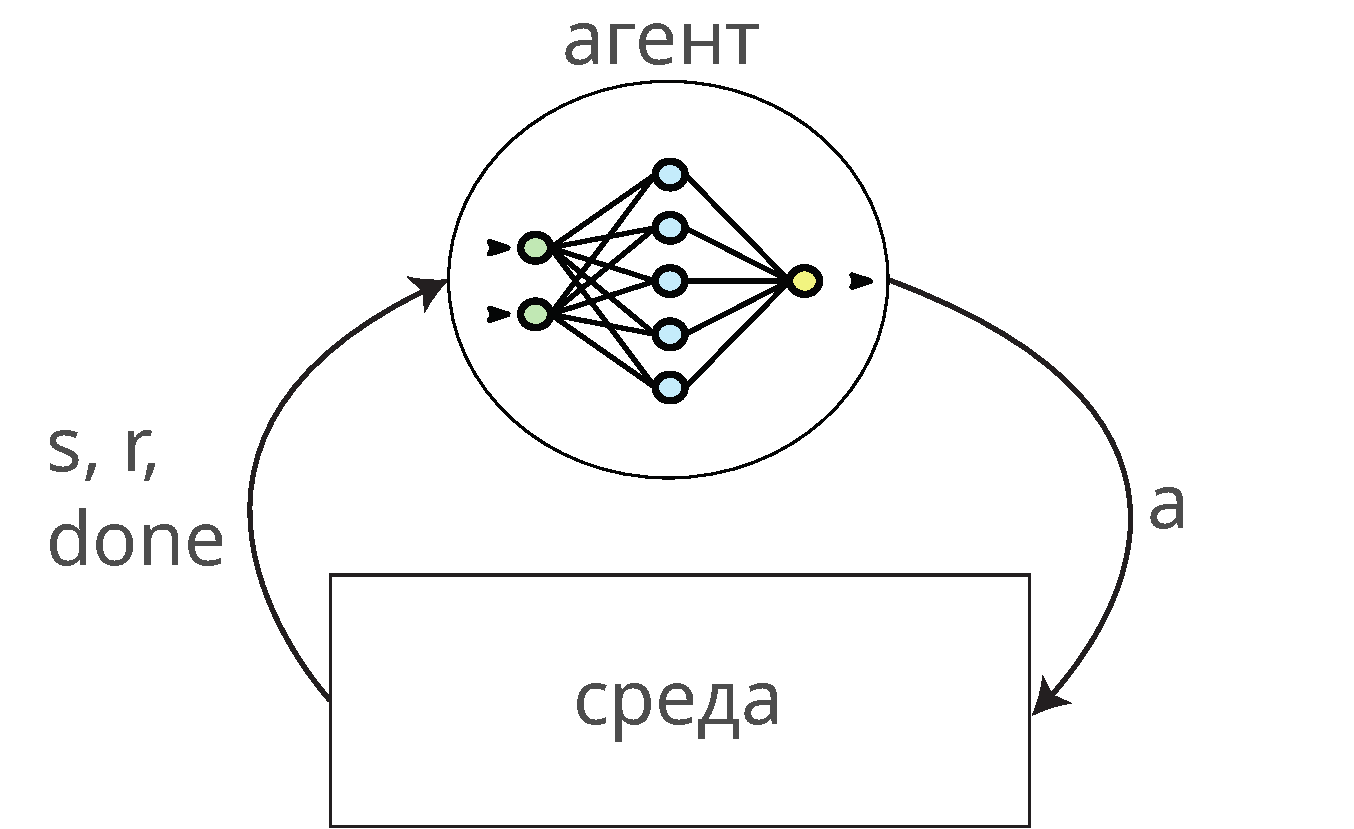
\includegraphics[width=1\linewidth]{Presentation/images/rl_setting_ru.pdf}
  \vspace{-10pt}
  \begin{equation*}
    <\mathcal{S, A, R, P}, \gamma>
  \end{equation*}

  \begin{align*}
  % & s_{t+1} \sim p(s_t, a) \\
  % & r_{t+1} = \mathcal{R}(s_t, a, s_{t+1}) \\
  % & \ex_{\tau \sim \pi} [G(\tau)] = \ex_{\tau \sim \pi} \left[r_0 + \gamma r_{1} + \gamma ^ 2 r_{2} + ...\right] \\
  & V^{\pi}(s_t) = \ex_{\tau \sim \pi}\left[\sum_{k=0}^{\infty} \gamma ^{k} r_{k+t}\right] \\
  & Q^{\pi}(s_t, a_t) = \ex_{\tau \sim \pi}\left[r_t + \sum_{k=0}^{\infty} \gamma ^{k + 1} r_{t + k + 1}\right] \\
  & \tau - \text{траектория}
  \end{align*}

\column{0.5\linewidth}
\centering
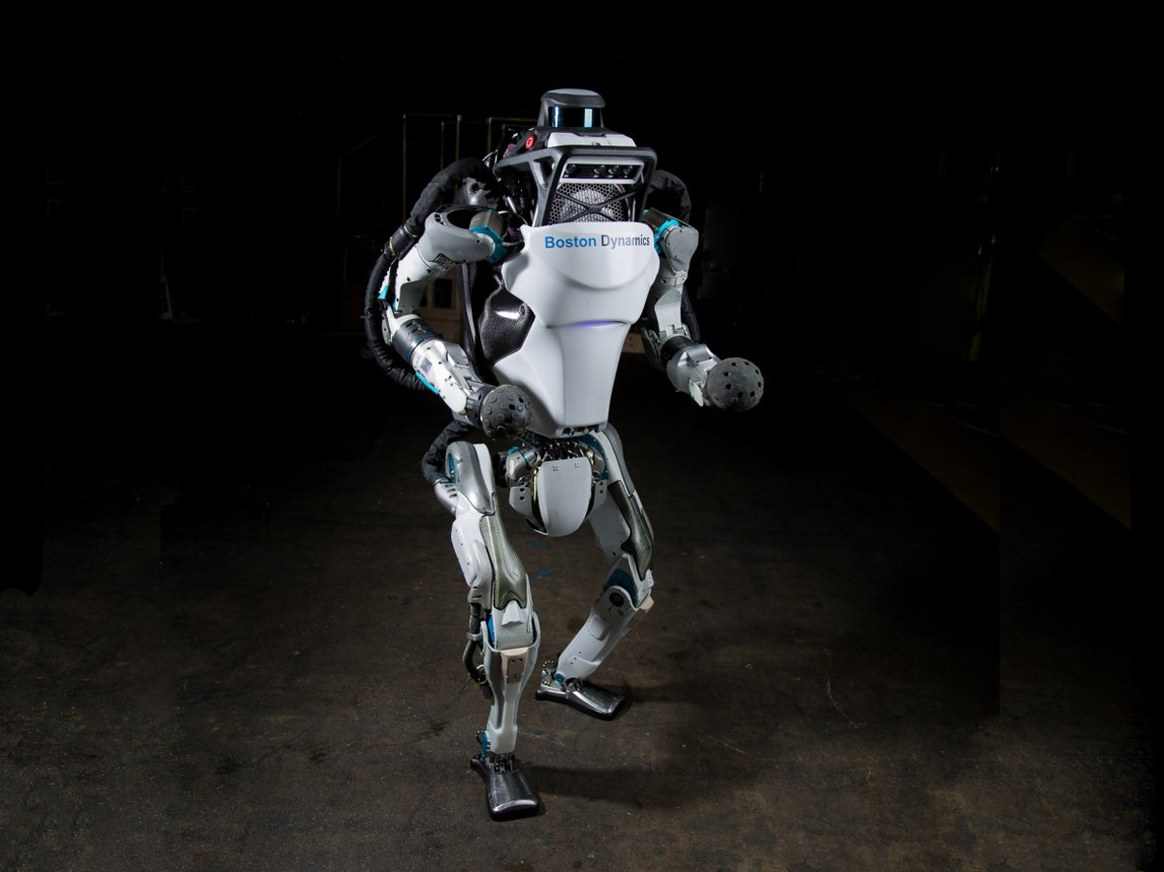
\includegraphics[width=0.8\linewidth]{Presentation/images/boston_dunamics.jpg}

\vspace{10pt}
\centering
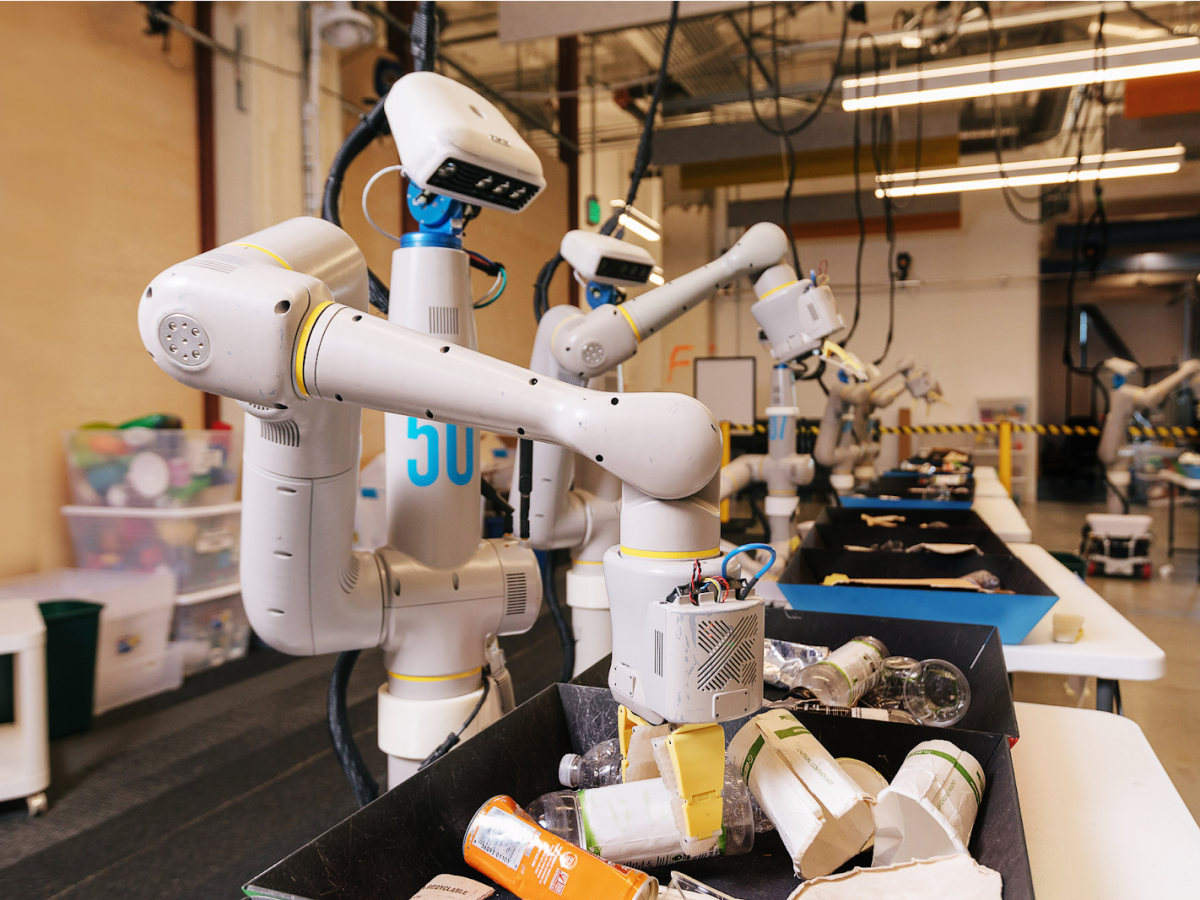
\includegraphics[width=0.8\linewidth]{Presentation/images/garbage_sorting.png}

\end{columns} 
\end{frame}

\begin{frame}
    \setlength{\leftmargini}{0cm}
    \frametitle{Цель работы}
     Развитие методов машинного обучения с подкреплением для решения задач управления робототехническими устройствами и виртуальными агентами.

    \vspace{20pt}
    В данный момент область применения методов RL ограничена:
    \begin{itemize}
        \item[] \textbf{Вызов 1.} Sim2Real gap, при переносе агента, обученного в симуляции, на физическую установку.
        \item[] \textbf{Вызов 2.} Сложности с моделированием стратегии $\pi$, которая использует действия различной амплитуды.
        \item[] \textbf{Вызов 3.} Сходимость стратегии к локальному  оптимуму при не оптимальной функции награды.
       \item[] \textbf{Вызов 4.} Сложности с объединением RL и классических алгоритмов в рамках иерархического агента.
    \end{itemize}
\end{frame}

\iffalse
\begin{frame}
    \frametitle{Положения, выносимые на защиту}
    \begin{itemize}
        \item Метод обучения с подкреплением способный оперировать действиями различного масштаба, устойчивый к шумам, и его применение для настройки оптического интерферометра.
        \item Программно-аппаратный комплекс автоматической настройки оптического интерферометра.
        \item Метод обучения стратегии для управления движением шагающего робота с заданной линейной и угловой скоростью.
        \item Иерархический алгоритм комбинирующий алгоритмический и нейросетевой подходы и его применение для управления агентом в среде NetHack.
    \end{itemize}
\end{frame}
\note{
    Проговариваются вслух положения, выносимые на защиту
}
\fi


\begin{frame}
    \frametitle{Задачи исследования}
    \begin{itemize} 
        \item \underline{Задача 1.} Разработка метода, способного оперировать действиями различного масштаба, устойчивого к шумам, и его применение для настройки оптического интерферометра (вызов 1,2).
        \item \underline{Задача 2.} Разработка метода, который позволяет достичь сходимости к хорошему оптимуму для многозадачного агента и его применение  для управления движением шагающего робота (вызов 3).
        \item \underline{Задача 3.} Разработка иерархического алгоритма, который комбинирует алгоритмический и нейросетевой подходы и его применение для управления агентом в среде NetHack (вызов 4).
    \end{itemize}
\end{frame}

      % Первые слайды презентации
\metroset{sectionpage=none}
\section{Глава 2. Разработка метода, способного оперировать действиями различного масштаба, устойчивого к шумам, и его применение для настройки оптического интерферометра 
}

\begin{frame}
    \frametitle{Задачи исследования}
    \begin{itemize} 
        {\color{orange}\item \underline{Задача 1.} Разработка метода, способного оперировать действиями различного масштаба, устойчивого к шумам, и его применение для настройки оптического интерферометра (вызов 1,2).}
        \item \underline{Задача 2.} Разработка метода, который позволяет достичь сходимости к хорошему оптимуму для многозадачного агента и его применение  для управления движением шагающего робота (вызов 3).
        \item \underline{Задача 3.} Разработка иерархического алгоритма, который комбинирует алгоритмический и нейросетевой подходы и его применение для управления агентом в среде NetHack (вызов 4).
    \end{itemize}
\end{frame}


\begin{frame}{Постановка задачи оптимизации}

$$Q(s_t,a_t) = \ex_{r_{t+1},s_{t+1}}\left[r_{t+1} + \gamma \max_{a^{\prime} \in \mathcal{A}}Q(s_{t+1},a^{\prime})\right]$$
$$\pi = \argmax_{a \in \mathcal{A}}Q(s,a)$$

Особенности:
\begin{enumerate}
    \item Произвольное начальное состояние $s_0 \in \mathcal{S}$.
    \item Оптимальная стратегия должна оперировать действиями различного масштаба $a \sim \pi^*(s): \color{red}{\min(|a|) \ll \max(|a|)}$.
    \item Высокая размерность пространства состояний $s \in \mathcal{R}^N$
    \item Перенос из симуляции на физическую установку.\\
    Обучение: \hspace{12pt}$p_{\mathrm{sim}}(s_{t+1}|s_t, a_t)$.\\
    Применение: ${\color{red}p_{\mathrm{exp}}}(s_{t+1}|s_t, a_t + {\color{red}\zeta})$.
\end{enumerate}
\end{frame}

\begin{frame}{Алгоритм 1: Подбор параметров симулятора и их рандомизация \footnotemark[1,2]}

\vspace{-10pt}
\begin{minipage}{\linewidth}

\begin{columns}
\column{0.5\linewidth}
Train: $p_{\mathrm{sim}}(s_{t+1}|s_t, a_t, \theta_1, ..., \theta_n)$
Test: \hspace{1pt} ${\color{red}p_{\mathrm{exp}}}(s_{t+1}|s_t, a_t + {\color{red}\zeta})$
\vspace{10pt}
\begin{enumerate}
    \item Подбирем средние значения параметров $\theta_1, ..., \theta_n$: $<s_{\mathrm{sim}}>$ $\sim$ $<s_{\exp}>$

    \item Зашумляем $\theta \gets [\theta_{\min}, \theta_{\max}]$ для устойчивости к шумам
\end{enumerate}

\column{0.6\linewidth}
\begin{algorithm}[H]
\KwData{
$<s_{\exp}> \sim p_{\exp}(s_{t+1}|s_t, a_t)$\\
\hspace{33pt}$<s_{\mathrm{sim}}> \sim p_{\mathrm{sim}}(s_{t+1}|s_t, a_t, \theta)$
}
\KwResult{$\theta_1, ..., \theta_n$} 
$\varepsilon \gets f(<s_{sim}>, <s_{\exp}>)$\;
\While{$\varepsilon > \varepsilon_{\min}$}{
  $\theta \gets$ optimize($\theta$)\;
  $<s_{\mathrm{sim}}> \sim p_{\mathrm{sim}}(s_{t+1}|s_t, a_t, \theta)$\;
  $\varepsilon \gets f(<s_{sim}>, <s_{\exp}>)$\;
}
\end{algorithm}
Подбор значений параметров $\theta$. 
\end{columns}
\end{minipage}

%\vspace{10pt}
\begin{minipage}{\linewidth}
\fontsize{8pt}{10pt}\selectfont
    \emph{Замечание}: Если агент устойчив к шуму в наблюдениях, то шум в действиях $a_t + \zeta$ не будет влиять на стратегию агента, если он является несмещенным $\ex (a_t + \zeta) = a_t$
\end{minipage}

\setcounter{footnote}{0} 
\footnotetext[1]{Peng, X. B., Andrychowicz, M., Zaremba, W., Abbeel, P. Sim-to-Real Transfer of Robotic Control with Dynamics Randomization. ICRA, 2018.}
\footnotetext[2]{Rao, K., Harris, C., Irpan, A., Levine, S., Ibarz, J., and Khansari, M. RL-CycleGAN: Reinforcement Learning Aware Simulation-to-Real. CVPR, 2020.}

\end{frame}

\setcounter{footnote}{0} 
\begin{frame}{Алгоритм 2: Масштабирование действий\footnotemark}

\vspace{-20pt}
\begin{minipage}{\linewidth}
\begin{columns}
\column{0.5\linewidth}
\begin{align*}
& a \in \mathcal{R}^n: a_i \in [-1, 1] \\
& \text{параметр } b \gg 1\\ 
& a_i^{\prime} =
   \begin{cases}
    {\mathrm{sign}}(a_i) \cdot b^{|a_i| - 1}, |a_i| > a_{\min}
    \\
    0
  \end{cases}
\end{align*}

\column{0.5\linewidth}
\begin{figure}
    \centering
    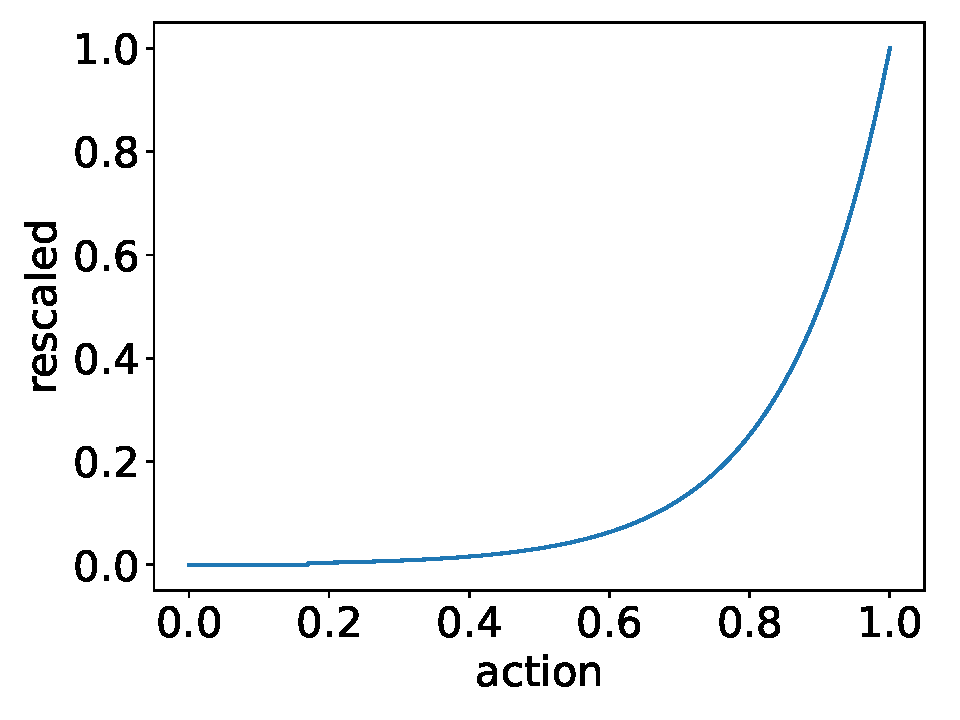
\includegraphics[width=1\linewidth]{images/rescale.pdf}
\end{figure}

\end{columns}
\end{minipage}

\vspace{-10pt}
\begin{minipage}{\linewidth}
\begin{columns}
\column{0.5\linewidth}
\centering Пример: CartPole Continous
\vspace{5pt}
    \begin{tabular}{c|c|c}
         & return & position \\ 
         \hline
         rescaled &  2756 $\pm$ 842 & -0.04 $\pm$ 0.09\\
         raw & 1692 $\pm$ 932 & 0.03 $\pm$ 0.22 
    \end{tabular}

\vspace{10pt}\hspace{-5pt} $r = -\log(|x| + 10^{-5})$  


\column{0.5\linewidth}
\begin{figure}
    \centering
    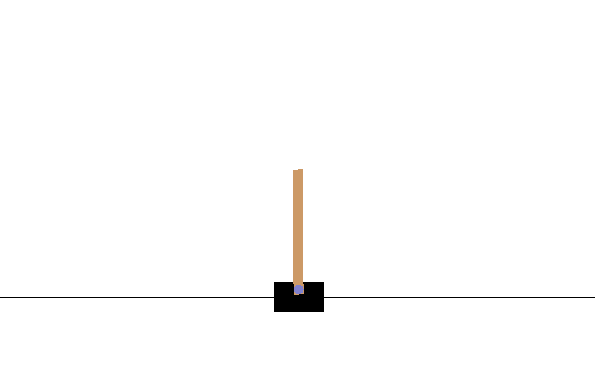
\includegraphics[width=0.8\linewidth]{Presentation/images/cartpole.png}
\end{figure}
\end{columns}
\end{minipage}

\footnotetext[1]{Dadashi, R., Hussenot, L., Vincent, D., Girgin, S., Raichuk, A., Geist, M., Pietquin, O. Continuous Control with Action Quantization from Demonstrations, ICML, 2022}

\end{frame}



\begin{frame}{Практическая задача: Настройка оптического интерферометра}
\vspace{-30pt}
\begin{figure}
  \centering
  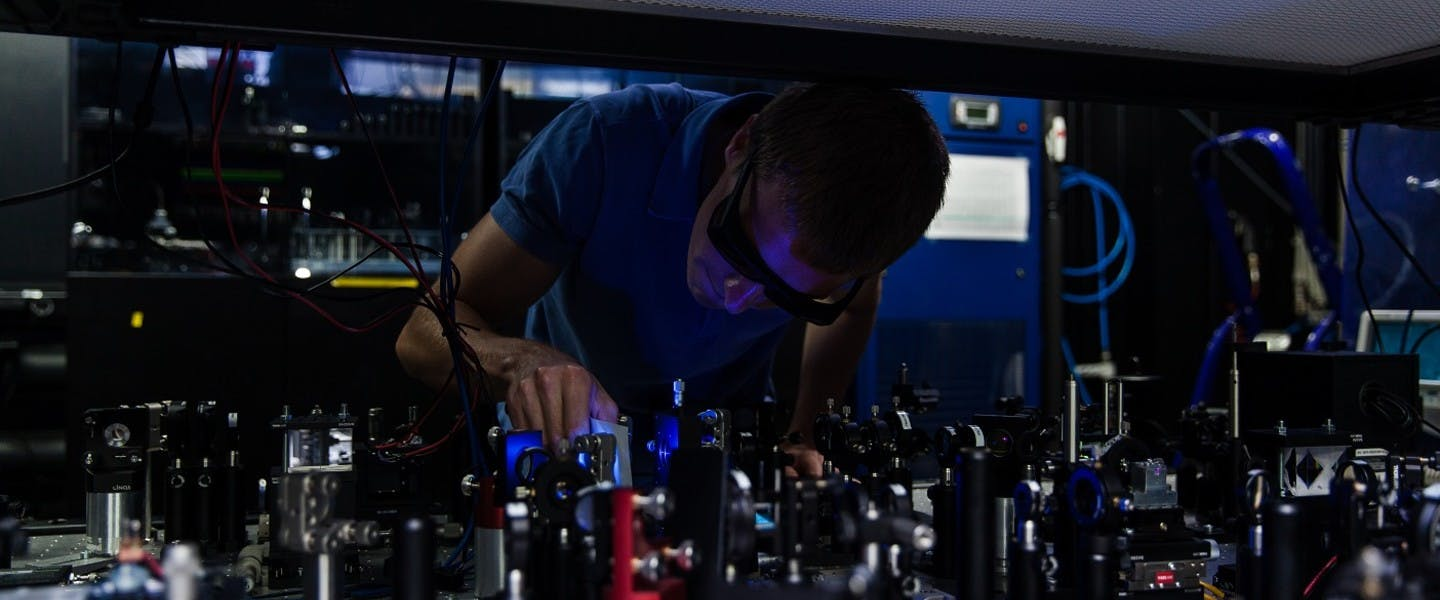
\includegraphics[width=1\linewidth]{Presentation/images/labinterf.jpg}
\end{figure}
\vspace{-10pt}

\setcounter{footnote}{0} 
Смежные задачи рассматривались в работах\footnotemark[1,2]\footnotetext[1]{Degrave, J., Felici, F., Buchli, J. et al. Magnetic control of tokamak plasmas through deep reinforcement learning. Nature, 2022.}
\footnotetext[2]{Chen, IJ., Aapro, M., Kipnis, A. et al. Precise atom manipulation through deep reinforcement learning. Nat Commun, 2022.}
\end{frame}

\subsection{Постановка задачи}

\begin{frame}
\frametitle{Физические принципы работы и модель оптического интерферометра}
\begin{columns}
\column{0.5\linewidth}
  \centering
  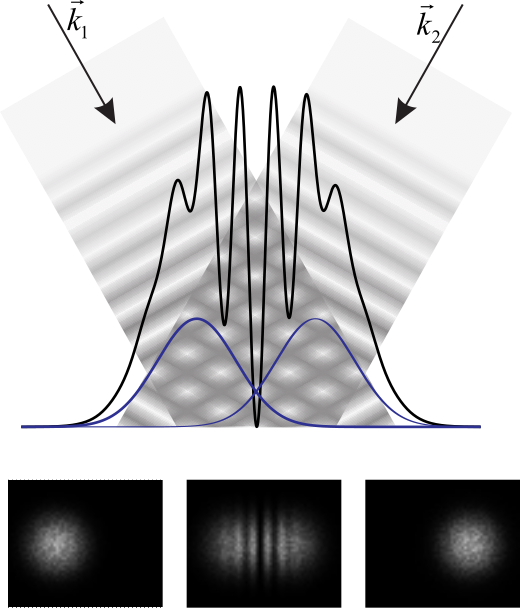
\includegraphics[width=0.9\linewidth]{images/interf_expl.png}

\column{0.5\linewidth}

\begin{align*}
& E(x,y,z)=\exp \left[-\frac{\left(x-x_{0}\right)^{2}+\left(y-y_{0}\right)^{2}}{r^{2}(z)}\right] \cdot \\
& \hspace{20pt} \exp \left[-i\left(k_{x} x+k_{y} y+k_{z} z + k\frac{x^2+y^2}{2\rho^2(z)} z\right)\right] \\
& E(x, y, z) = E_1(x, y, z) + E_2(x, y, z) \\
& I(x, y, z) = |E(x, y, z)|^2 = E(x,y,z) \cdot E^*(x,y,z) \\
& I= I_1 + I_2 + 2 \sqrt{I_1I_2}\cos(\Delta \phi)
\end{align*}

\end{columns} 
\end{frame}

\begin{frame}
\frametitle{Интерферометр Маха-Цендера}
  \centering
  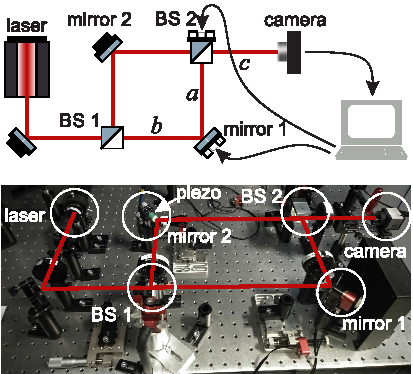
\includegraphics[width=0.8\linewidth]{scheme_with_experiment.pdf}
\end{frame}


\begin{frame}
\frametitle{Математическая модель интерферометра Маха-Цендера}
\begin{minipage}{\textwidth}
\begin{columns}
\column{0.6\linewidth}
  \centering
  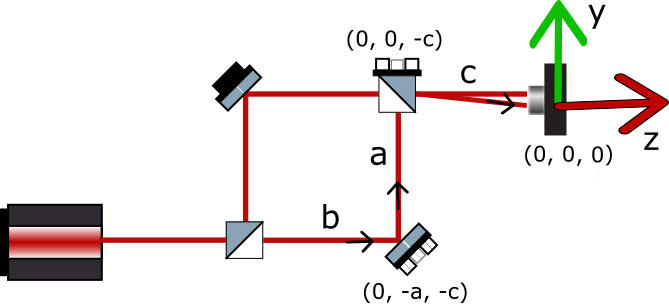
\includegraphics[width=1\linewidth]{Presentation/images/MZI_matmodel_v2.png}
  
\column{0.5\linewidth}
\begin{itemize}
    \item управление положением луча на камере $(x_0, y_0)$
    \item управление направлением $\vec{k}$
  \end{itemize}
\end{columns}
\end{minipage}

\vspace{20pt}

\begin{minipage}{\textwidth}
\begin{columns}
\column{0.6\linewidth}
  \centering
  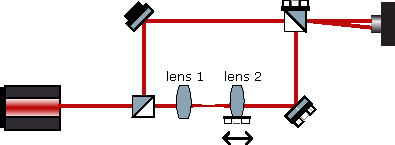
\includegraphics[width=1\linewidth]{images/MZI_expl_lenses.pdf}
  
\column{0.5\linewidth}
\begin{itemize}
    \item \textcolor{red}{управление волновым фронтом}
  \end{itemize}
\end{columns}
\end{minipage}
\end{frame}


\begin{frame}{Численная модель интерферометра Маха-Цендера}
\begin{columns}
\column{0.5\linewidth}
\centering
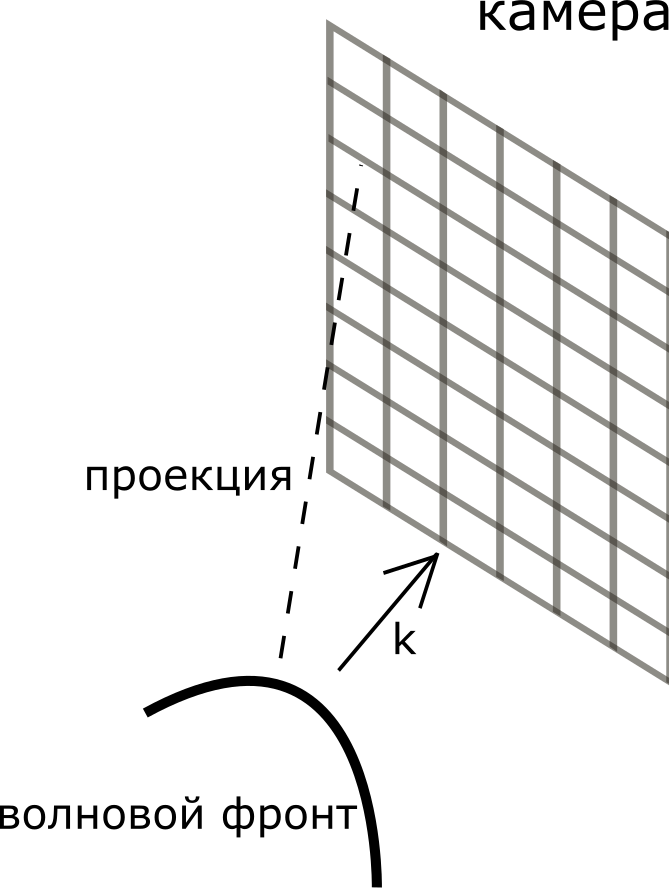
\includegraphics[width=0.8\linewidth]{images/wave_front_projection.png}
\column{0.5\linewidth}
\begin{enumerate}
    \item трассировка лучей 
    \begin{itemize}
        \item прохождение через зеркала $\vec{k}$, $(x_0, y_0)$
        \item радиус $r(z)$ и волновой фронт $\rho(z)$
    \end{itemize}
    \item вычисление интерференционной картины
    \begin{itemize}
        \item пространственное разрешение 64×64 пикселя
        \item временное разрешение 16 кадров
        \item параллельно для каждого пикселя и кадра
    \end{itemize}

    
\end{enumerate}

\end{columns}
\end{frame}



\begin{frame}
\frametitle{Интерференционная картина, полученная в эксперименте}
\begin{minipage}{\textwidth}

\begin{equation*}
\hspace{1000pt minus 1fil}
\text{Видность интерференционной картины }
    V = \frac{            
        \max_{t}(I_{\mathrm{tot}}) - \min_t(I_{\mathrm{tot}})}
        {\max_{t}(I_{\mathrm{tot}}) + \min_t(I_{\mathrm{tot}})}
\hfilneg
\end{equation*}
\end{minipage}

\begin{minipage}{\textwidth}
\begin{columns}
\column{0.7\linewidth}
\centering
    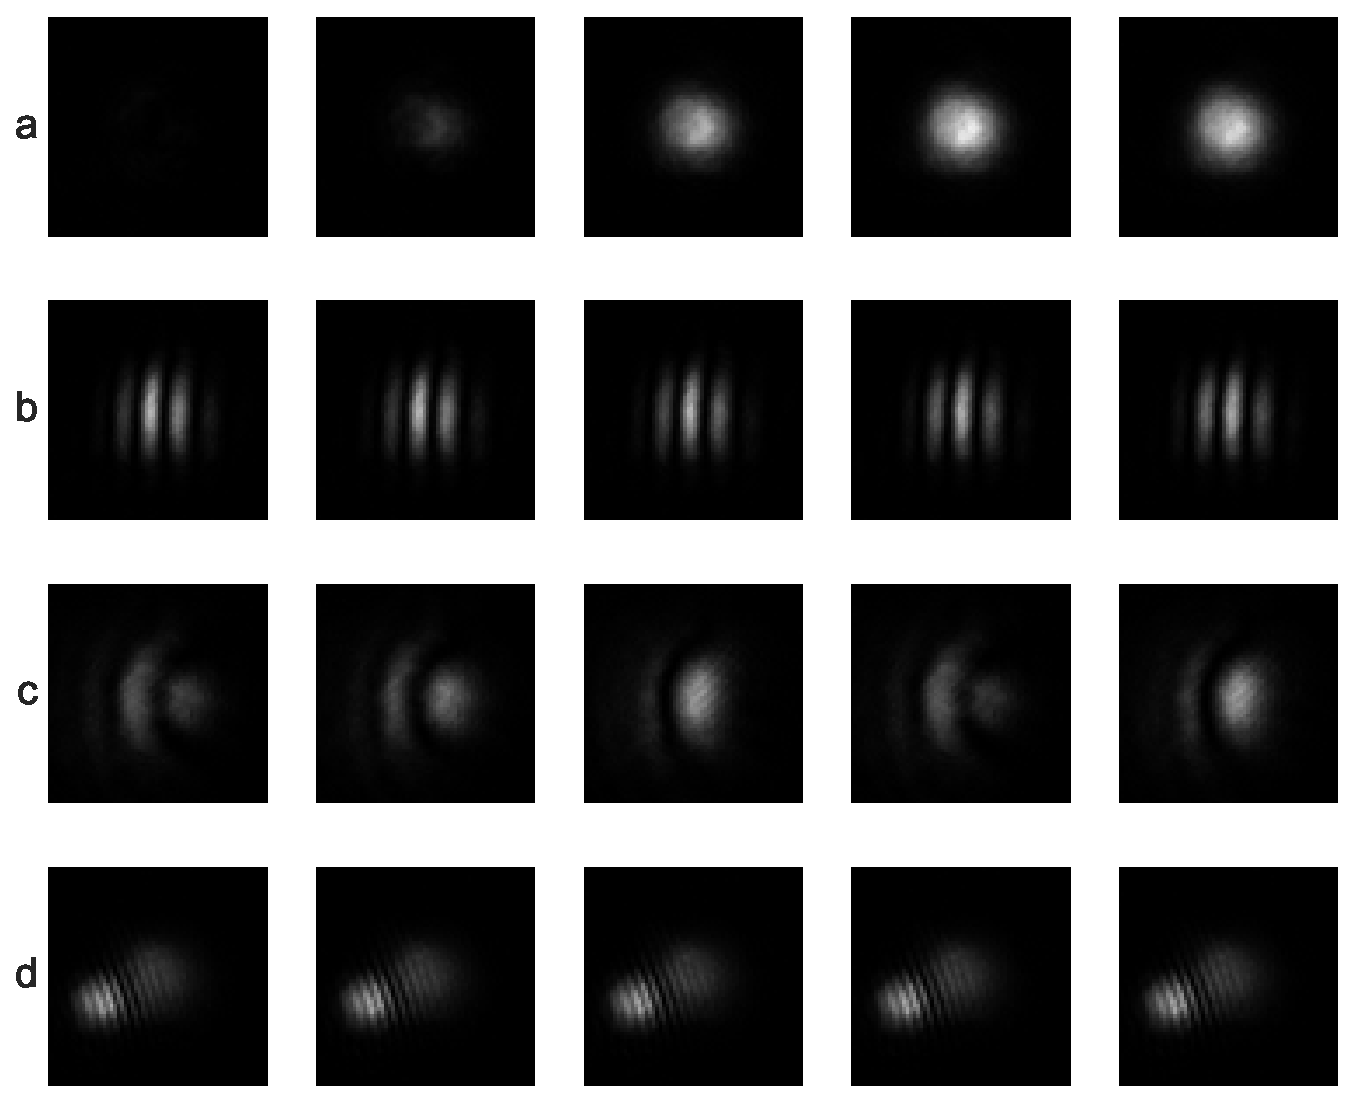
\includegraphics[width=1\linewidth]{images/Env_patterns.pdf}
\column{0.5\linewidth}
\begin{itemize}
    \item[] $V \approx 1$
    \vspace{30pt}
    \item[] $V \approx 0$
    \vspace{30pt}
    \item[] $V \approx 0.1$
    \vspace{30pt}
    \item[] $V \approx 0$
\end{itemize}
\end{columns}
\end{minipage}
    
\end{frame}




\subsection{Метод способный оперировать
действиями различного масштаба и устойчивый к оптическим
шумам}


\begin{frame}{Метод настройки, основанный на алгоритме DQN}
\begin{columns}
\column{0.5\linewidth}
\centering
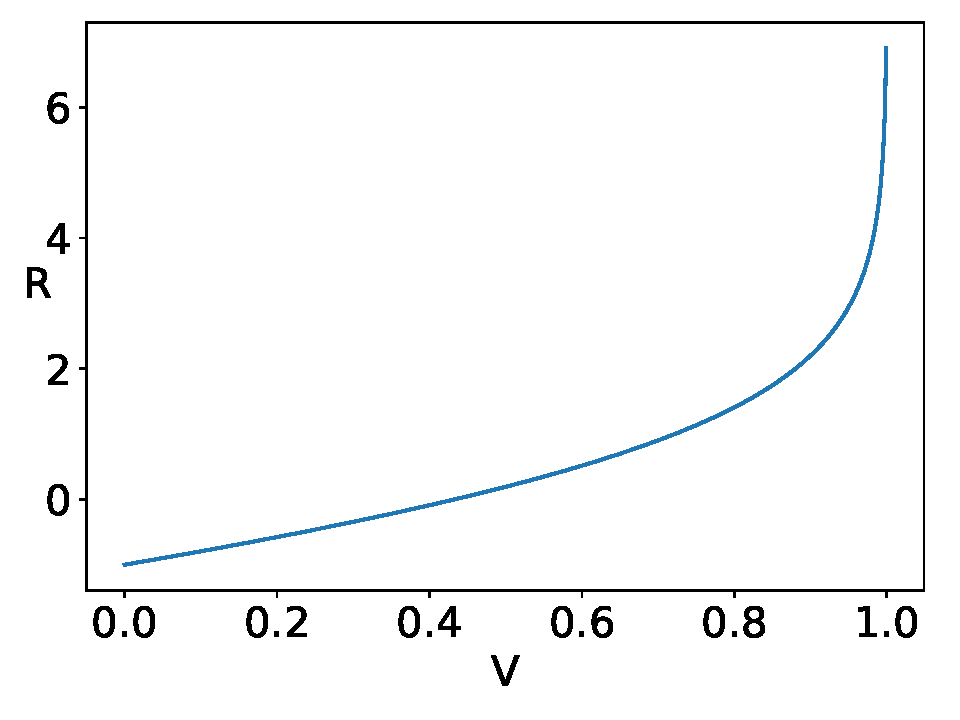
\includegraphics[width=1\linewidth]{images/reward_visib.pdf}
\column{0.5\linewidth}
\textbf{Награда}\\
$R = V - \log(1-V) - 1$\\
$V = 0.95 \to R = 2.9$\\
$V = 0.98 \to R = 3.9$\\
\textbf{Энкодер}\\
3-слойная сверточная  сеть [(32, 8, 4), (64, 4, 2), (64, 3, 1)] (Nature Mnih et.al, 2015)
\end{columns}
\vspace{10pt}
\textbf{Пространство наблюдений} 16 кадров 64x64 пикселя\\
\textbf{Пространство действий} \textcolor{red}{дискретное} (25/31) \\
\textbf{Эпизод} 100 шагов, случайный reset $\pm \alpha_{\mathrm{max}}$, $\pm \Delta_{\mathrm{max}}$\\
\textbf{Параметры} $\gamma = 0.99 \to  \Delta = \frac{1}{1 - \gamma} = \textcolor{red}{100}$, total steps $10^8$, buffer size $10^6$, batch size $32$\\

\end{frame}

\begin{frame}{Метод настройки, основанный на алгоритме TD3}
\begin{columns}
\column{0.5\linewidth}
\centering
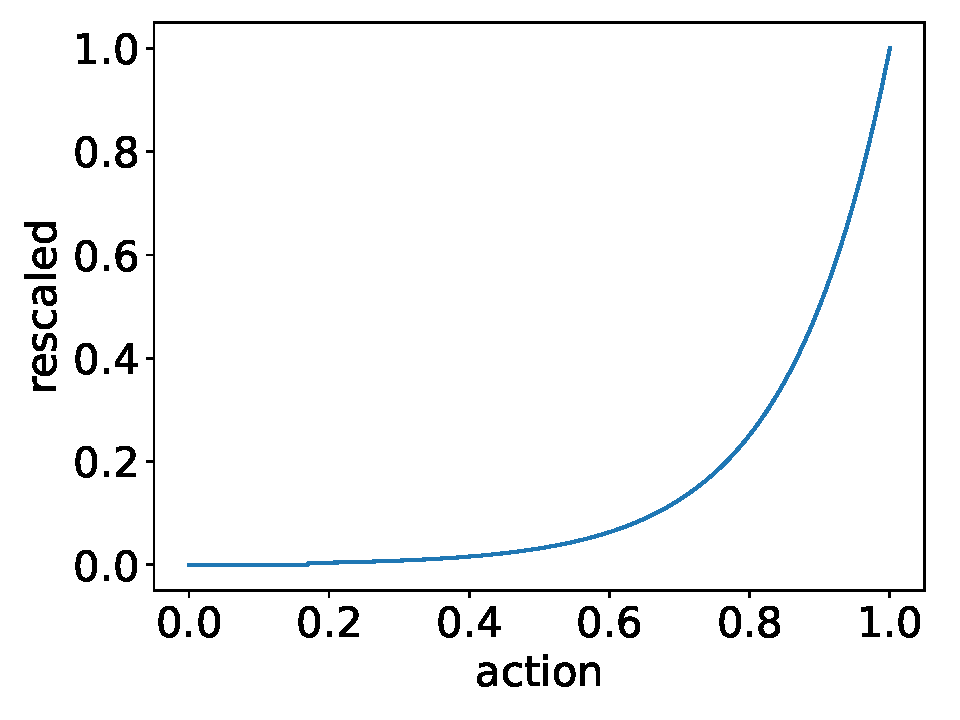
\includegraphics[width=1\linewidth]{images/rescale.pdf}
\column{0.5\linewidth}
\textbf{Награда}\\
$R = V - \log(1-V)$\\
\textbf{Масштабирование действий}\\
\vspace{-15pt}
\begin{equation*}
a^{\prime} =
   \begin{cases}
    {\mathrm{sign}}(a) \cdot 1000^{|a| - 1}, |a| > 0.17
    \\
    0
  \end{cases}
\end{equation*}
\textbf{Энкодер}\\
VGG-16
\end{columns}
\vspace{10pt}
\textbf{Пространство действий} \textcolor{red}{непрерывное} ($\mathcal{R}^4$/$\mathcal{R}^5$)\\
\textbf{Параметры} $\gamma = 0.8 \to  \Delta = \frac{1}{1 - \gamma} = \textcolor{red}{5}$, total steps $10^6$, buffer size $10^5$, batch size $32$ \\

\end{frame}

\begin{frame}{Перенос из симуляции в реальность}
\begin{columns}
\column{0.4\linewidth}
\centering
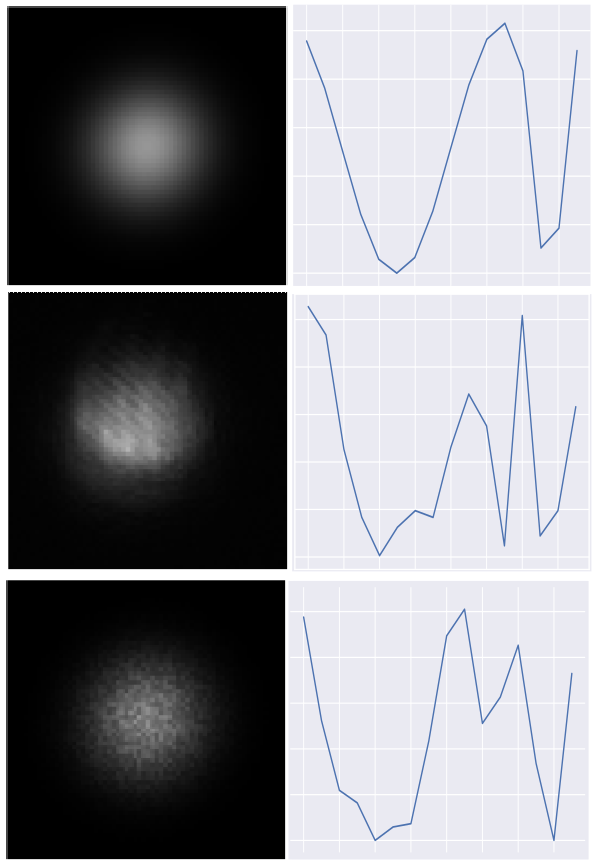
\includegraphics[width=1\linewidth]{beamsamples.png}
\column{0.6\linewidth}
\textbf{в начале каждого эпизода}
\begin{itemize}
    \item рандомизация радиуса пучка $\pm 20\%$
\end{itemize}
\textbf{на каждом шаге}
\begin{itemize}
    \item рандомизация времени выдержки камеры $\pm 30\%$
    \item шум в изображениях $20\%$
    \item циклический сдвиг кадров
    \item рандомизация движения пьезо зеркала
    \item фазовый шум $\phi \sim \mathcal{N}(\frac{2\pi k}{N}, 0.5)$
\end{itemize}
\end{columns}
\end{frame}

\subsection{Программно-аппаратный комплекс Интерферобот}

\begin{frame}{Программно-аппаратный комплекс Интерферобот}
\begin{columns}
\column{0.35\linewidth}
\centering
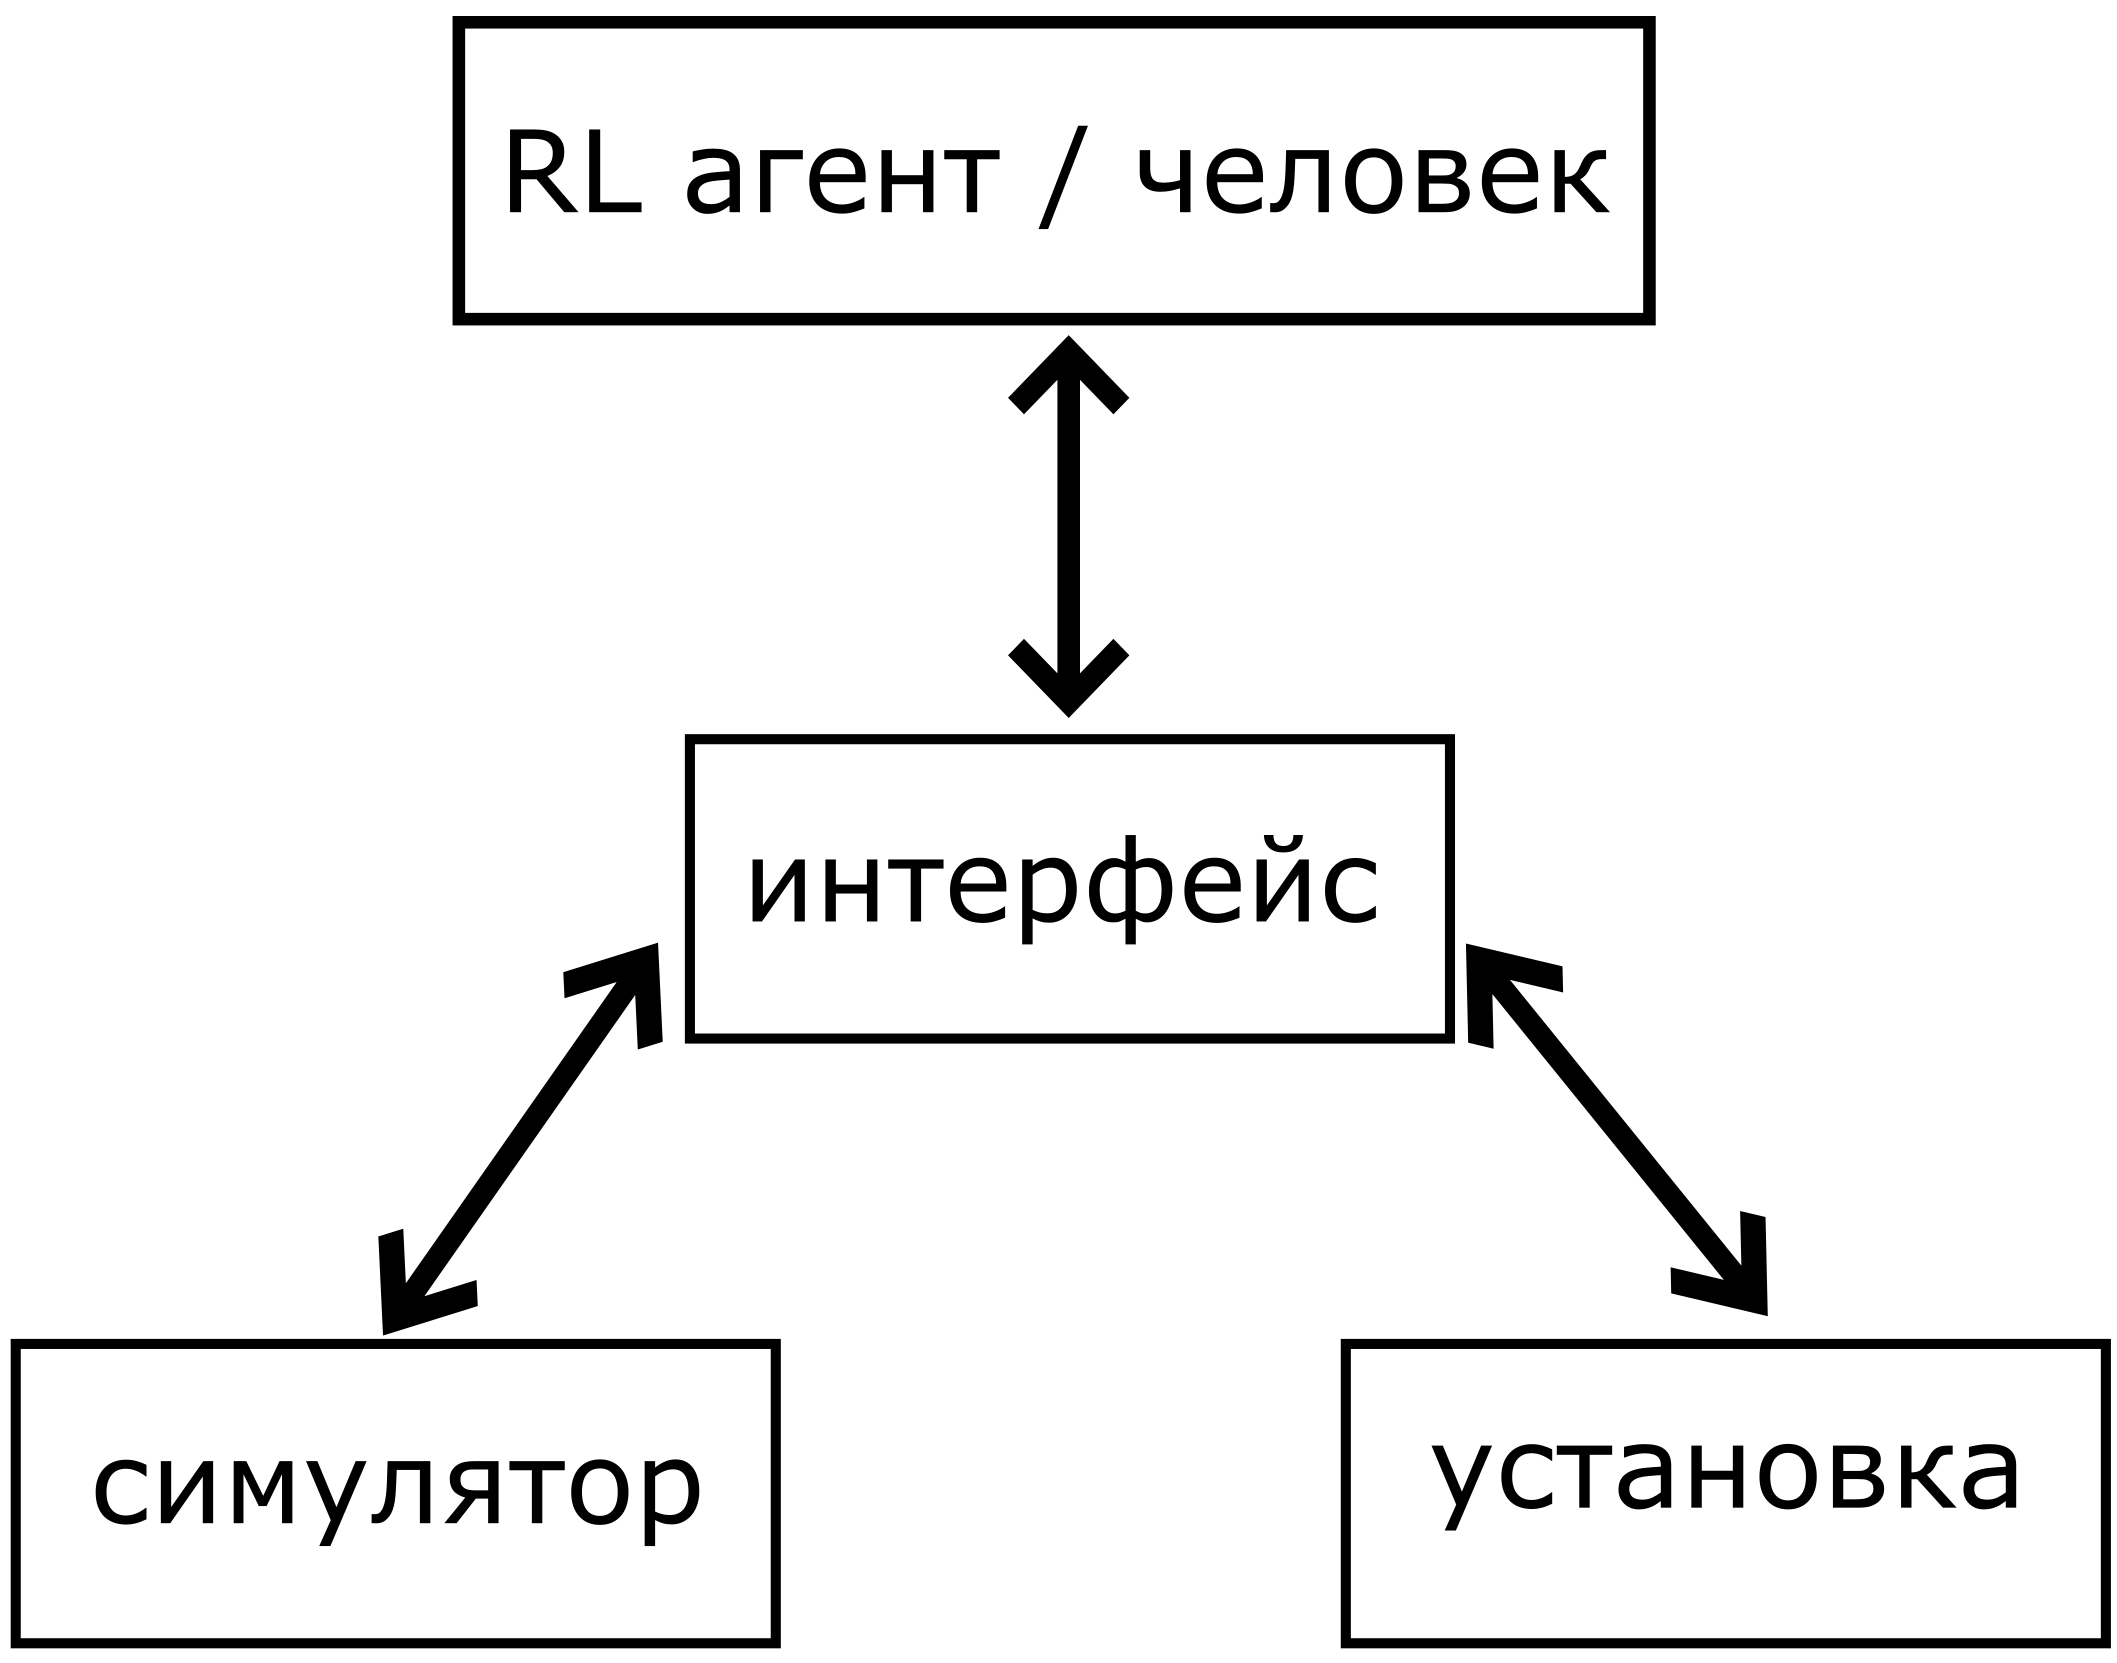
\includegraphics[width=1\linewidth]{images/interferobot_complex.png}
Схема взаимодействия модулей
\column{0.65\linewidth}
\centering
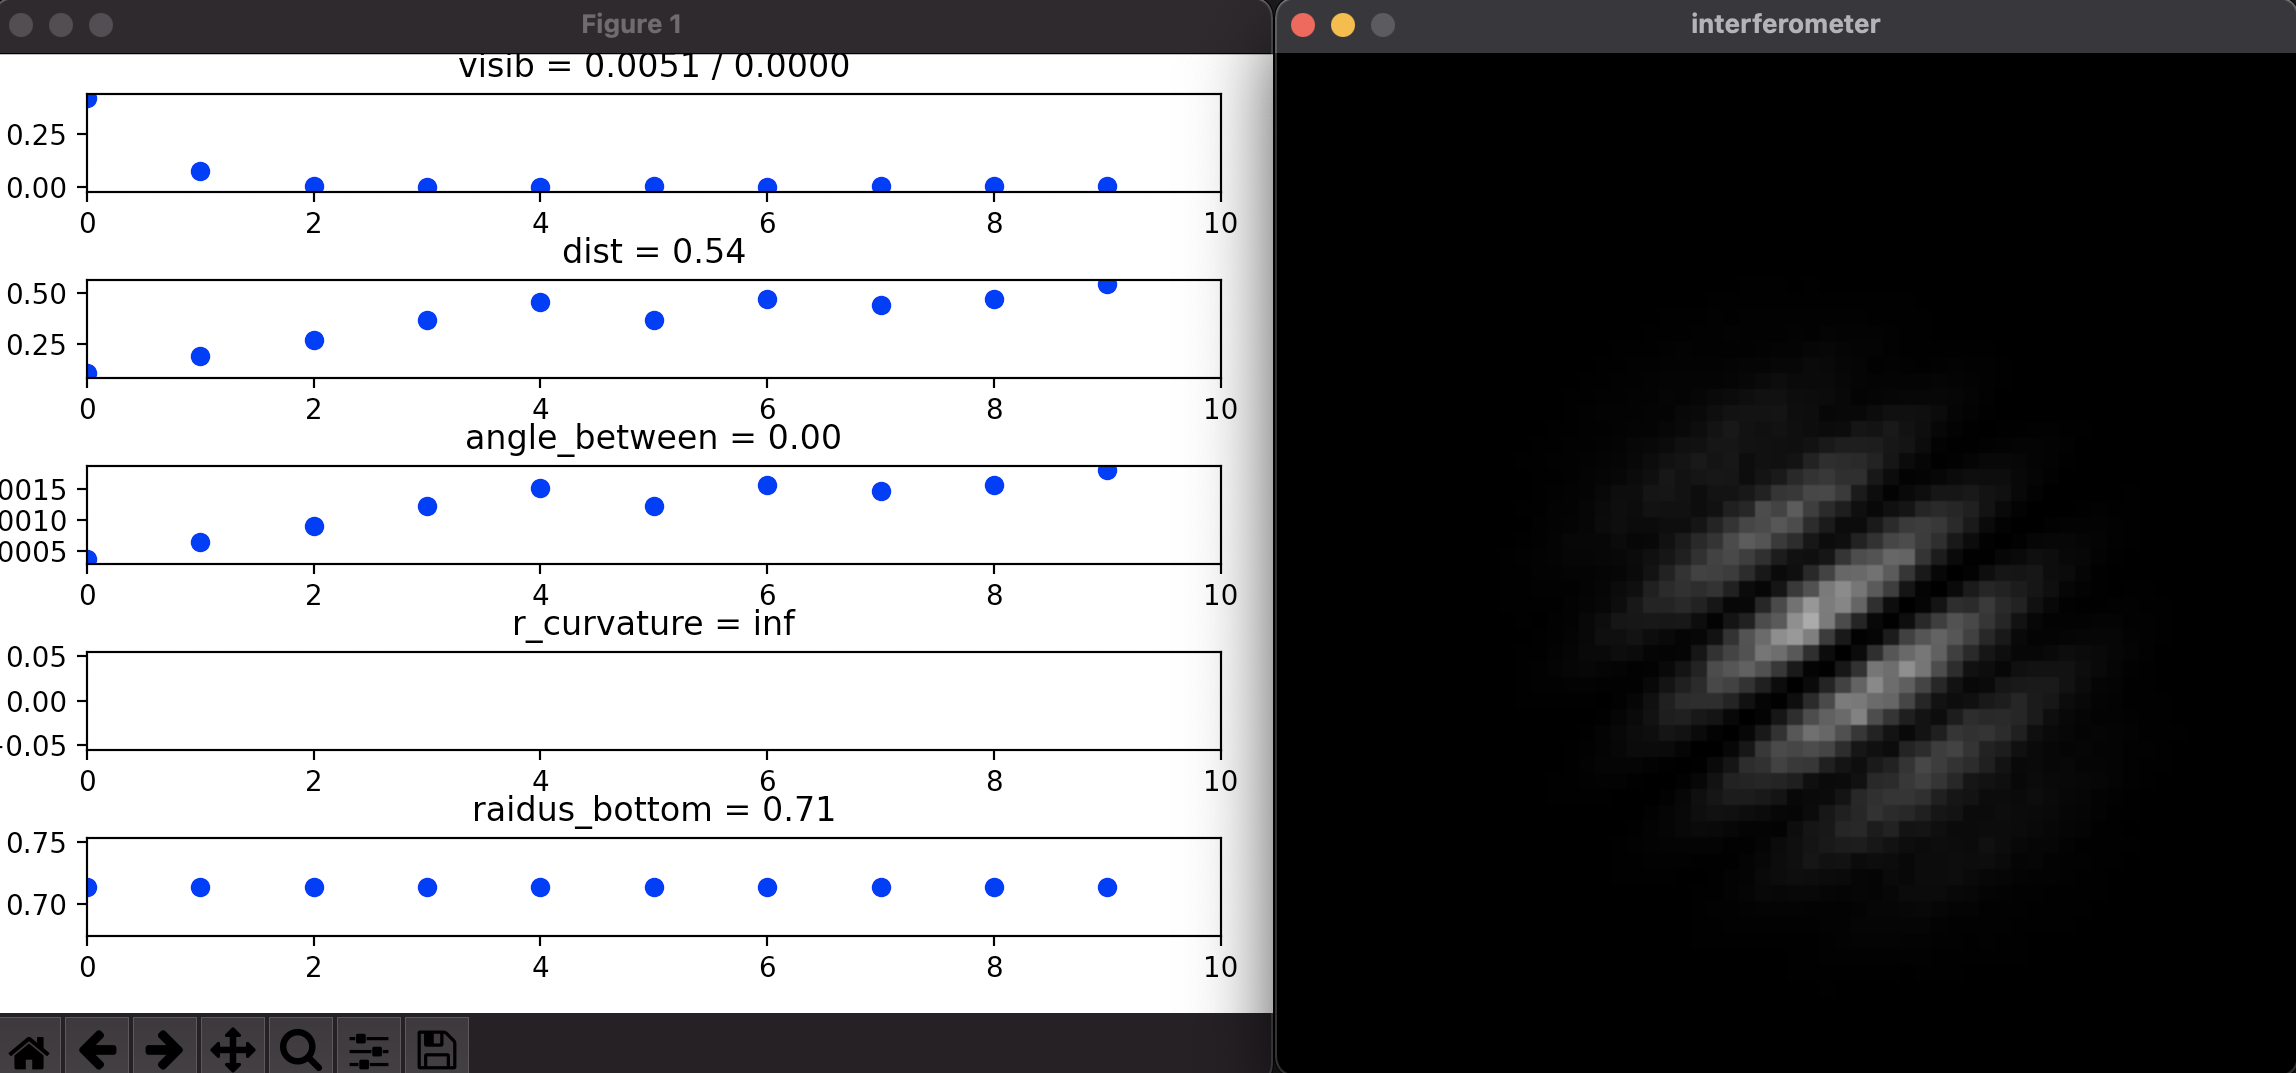
\includegraphics[width=1\linewidth]{images/gui.png}
Графический интерфейс пользователя
\end{columns}
\vspace{15pt}
C++, Python3\\
200 состояний среды (16x64х64) за одну секунду (16 потоков на intel core i7)
\end{frame}

\begin{frame}[allowframebreaks]{Настройка интерферометра Маха-Цендера без линз}
\begin{columns}
\column{0.5\linewidth}
\centering
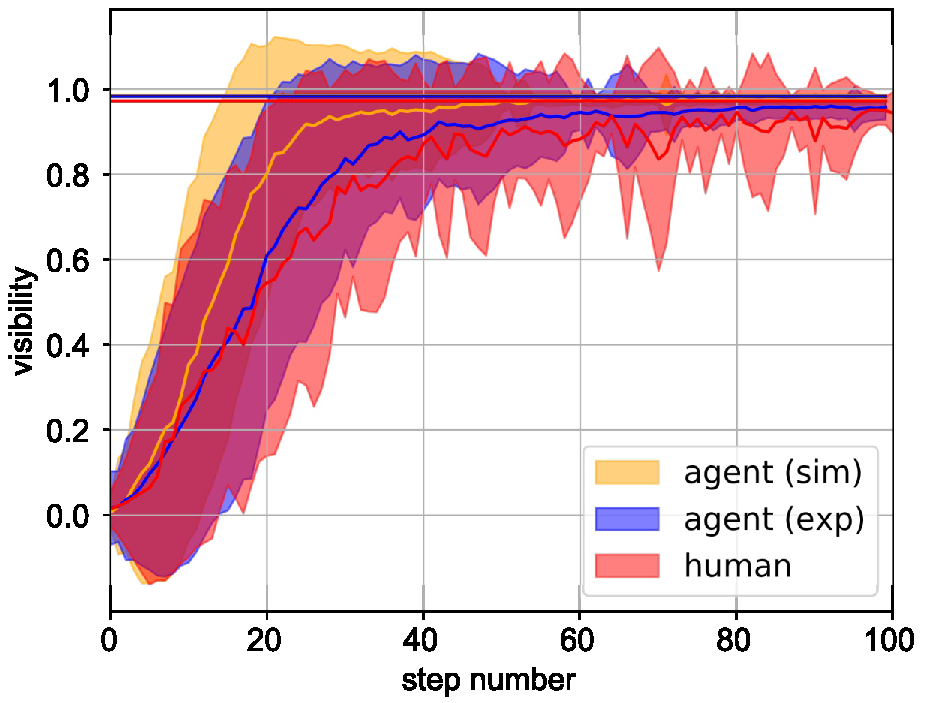
\includegraphics[width=1\linewidth]{images/eval1_visib_step.pdf}
\column{0.5\linewidth}
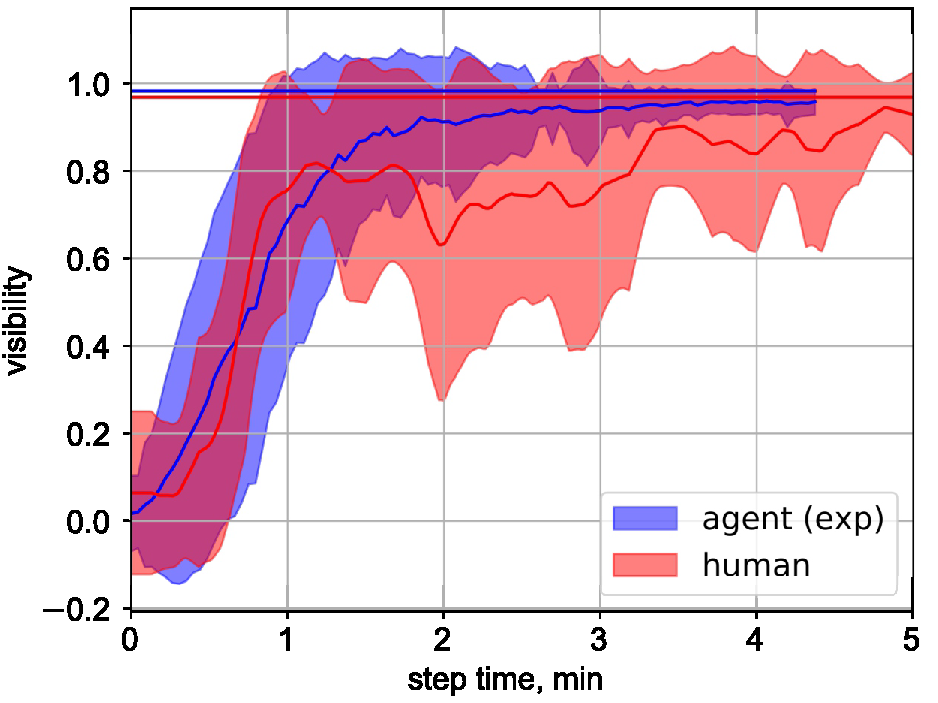
\includegraphics[width=1\linewidth]{images/eval1_visib_time.pdf}
\end{columns}

\vspace{-10pt}

\begin{table} [htbp]
    \centering
    \begin{threeparttable}
        \caption*{Средняя наибольшая видность достигнутая при настройке}
        \begin{tabular}{| p{3cm} || p{3cm} || p{3cm} |}
            \hline
            \hline
            DQN (sim) & DQN (exp) & Human \\
            \hline
            0.986 & 0.983 & 0.972 \\
            \hline
            \hline
        \end{tabular}
    \end{threeparttable}
\end{table}

\centering {\color{orange}Вывод:} дискретный агент работает на уровне опытного специалиста.

\framebreak 

\begin{table} [htbp]
    \centering
    \begin{threeparttable}
        \caption*{{\color{orange} Проверка идеи 1:} Анализ влияния шумов, используемых при обучении агента, на качество настройки физической установки}
        \begin{tabular}{| p{6cm} || p{2cm} || p{2cm} |}
            \hline
            \hline
             & видность & награда \\
            \hline
            Все рандомизации  & $\textbf{0.96} \pm \textbf{0.02}$ & $\textbf{221} \pm \textbf{54}$ \\
            Без рандомизации радиуса & $0.74 \pm 0.20$ & $85 \pm 69$ \\
            Без рандомизации выдержки & $0.91 \pm 0.04$ & $178 \pm 39$ \\
            Без шума в изображениях & $0.82 \pm 0.07$ & $129 \pm 43$ \\
            Без шума в движении пьезо зеркала &  $0.89 \pm 0.07$ & $200 \pm 42$ \\
            \hline
            \hline
        \end{tabular}
    \end{threeparttable}
\end{table}
\end{frame}

\begin{frame}[allowframebreaks]{Настройка интерферометра Маха-Цендера с системой линз}
\begin{columns}
\column{0.5\linewidth}
\centering
\includegraphics[width=1\linewidth]{Presentation/images/DQN_vs_TD3.png}
\column{0.5\linewidth}
\centering
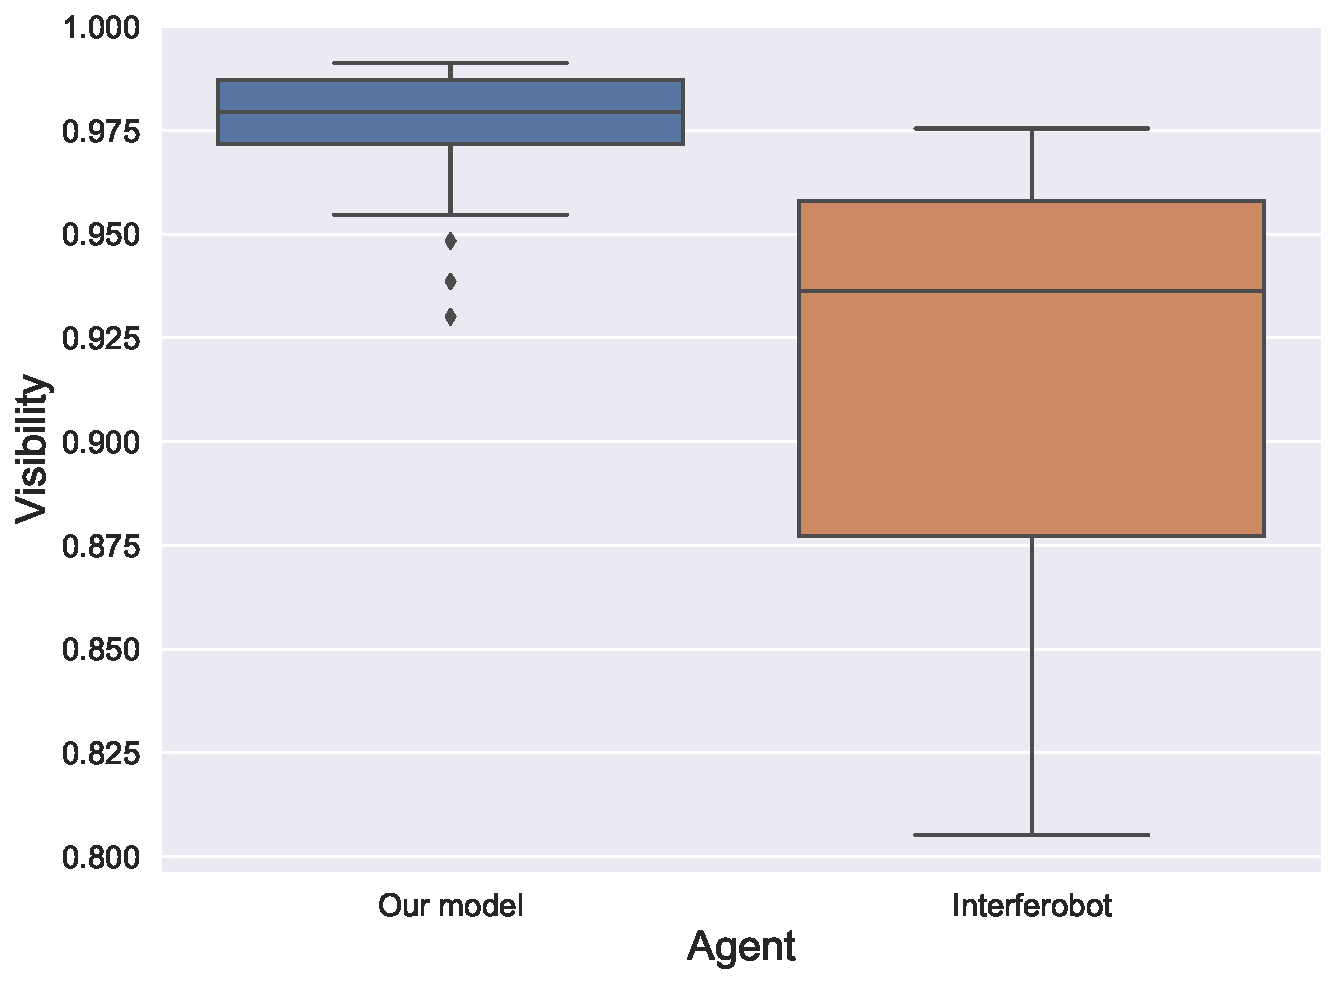
\includegraphics[width=1\linewidth]{images/DQN_vs_TD3_box.pdf}
\end{columns}

\vspace{-10pt}
\begin{table} [htbp]
    \centering
    \begin{threeparttable}
        \begin{tabular}{| p{2cm} || p{2cm} || p{2cm} || p{3cm} |}
            \hline
            \hline
            &V $\ge 0.92$ & V $\ge 0.95$ & V $\ge 0.98$ \\
            \hline
            Human &  93.9 (\textbf{0\%})  & 103.6 (\textbf{0\%}) & 129.6 (10\%)\\
            TD3 &  \textbf{56.16} (\textbf{0\%}) & \textbf{75.06} (\textbf{0\%}) & \textbf{120.1} (\textbf{4\%})\\
            DQN &  98.7 (7.6\%) & 116.1 (7.6\%) & 156.4 (10.6\%)\\
            \hline
            \hline
        \end{tabular}
    \end{threeparttable}
\end{table}

\centering {\color{orange}Вывод:} непрерывный агент работает лучше опытного специалиста.

\framebreak

\begin{table} [htbp]
    \centering
    \begin{threeparttable}
        \caption*{{\color{orange}Проверка идеи 2:} Анализ эффективности фазового шума и масштабирования действий. PN: фазовый шум, AR: масштабирование действий.}
        \begin{tabular}{| p{3cm} || p{3cm} || p{3cm} |}
            \hline
            \hline
            агент & средняя видность за последние 40 шагов & стандартное отклонение \\
            \hline
            TD3 + AR + PN & \textbf{0.98} & \textbf{0.03} \\
            TD3 + AR & 0.95 & 0.06\\
            DQN + PN & 0.90 & 0.08\\
            TD3& 0.83 & 0.18\\
            \hline
            \hline
        \end{tabular}
    \end{threeparttable}
\end{table}

\end{frame}

\begin{frame}{Пример настройки}
\begin{columns}
\column{0.5\linewidth}
    \centering
    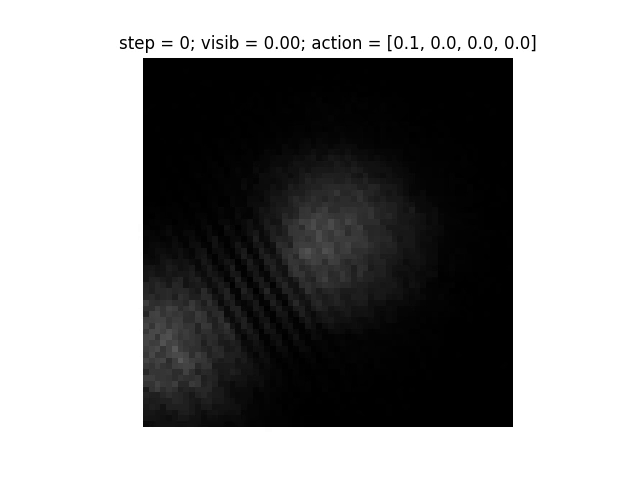
\includegraphics[width=1\linewidth]{Presentation/images/dqn_1.png}
    Дискретный DQN агент
\column{0.5\linewidth}
    \centering
    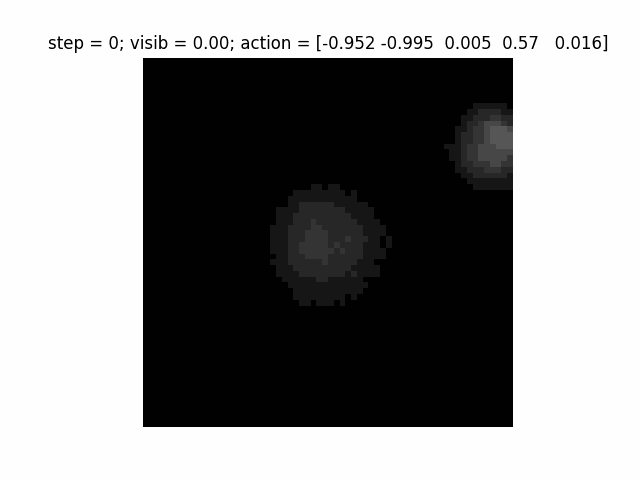
\includegraphics[width=1\linewidth]{Presentation/images/td3_1.png}
    Непрерывный TD3 агент
\end{columns}
\end{frame}


\begin{frame}{Результаты задачи 1}
\begin{itemize}
    \item[\textcolor{ForestGreen}{\checkmark}] Разработаны алгоритмы, подбора параметров симуляции и масштабирования пространства действий. 
    \item[\textcolor{ForestGreen}{\checkmark}] На основе предложенных алгоритмов реализованы методы настройки оптического интерферометра основанные на обучении с подкреплением.
    \begin{itemize}
        \item[--] Разработан симулятор интерферометра Маха-Цендера.
        \item[--] Разработан программно-аппаратный комплекс Интерферобот.
        \item[--] Предложен набор шумов и функция награды.
        \item[--] Качество настройки с использованием разработанного метода превосходит качество настройки эксперта.
    \end{itemize}
    
    
\end{itemize}
    



\end{frame}

% \subsection{Не нумерованные}


\section{Глава 3. Метод управления линейной и угловой скоростью шагающего робота основанный на обучении с подкреплением}

\begin{frame}
    \frametitle{Задачи исследования}
    \begin{itemize} 
        \item \underline{Задача 1.} Разработка метода, способного оперировать действиями различного масштаба, устойчивого к шумам, и его применение для настройки оптического интерферометра (вызов 1,2).
        {\color{orange}\item \underline{Задача 2.} Разработка метода, который позволяет достичь сходимости к хорошему оптимуму для многозадачного агента и его применение  для управления движением шагающего робота (вызов 3).}
        \item \underline{Задача 3.} Разработка иерархического алгоритма, который комбинирует алгоритмический и нейросетевой подходы и его применение для управления агентом в среде NetHack (вызов 4).
    \end{itemize}
\end{frame}

\begin{frame}{Постановка задачи оптимизации}

$$V(s_t) = \max_{a \in \mathcal{A}}\ex_{r_{t+1},s_{t+1}}\left[r_{t+1} + \gamma V(s_{t+1})\right]$$
$$\pi(s_t) = \argmax_{a \in \mathcal{A}}\ex_{r_{t+1},s_{t+1}}\left[r_{t+1} + \gamma V(s_{t+1})\right]$$

Особенности:
\begin{enumerate}
    \item Многозадачность - хотим решать несколько задач с помощью единого агента.
    \item Сложная функция награды - сходимость к суб-оптимальной стратегии. 
    \item Высокая размерность пространства состояний $s \in \mathcal{R}^N$.
\end{enumerate}
\end{frame}

\begin{frame}{Алгоритм: обучение по расписанию для многозадачного агента}

\begin{minipage}{\linewidth}

\begin{columns}
\column{0.5\linewidth}
\begin{enumerate}
    \item Для многозадачности будем рассматривать каждую задачу как часть состояния агента $s = (o, t)$, $t$ - текущая задача. 
    \item Будем увеличивать штрафные коэффициенты в функции награды линейно по мере обучения агента:
    \vspace{-10pt}
    \begin{equation*}
        r = r_{task} - \frac{n}{N} \cdot \sum_i r_{\mathrm{penalty}_i}
    \end{equation*}
\end{enumerate}

\column{0.5\linewidth}
\begin{algorithm}[H]
\KwData{
распределение задач $T$
}
\KwResult{параметры агента $\theta$} 
\While{n < $N$}{
  выбираем задачи $t_i \sim T$\;
  \ForEach {$t_i$} {
    генерируем траекторию $\tau \sim \pi_{\theta}(\cdot |t_i)$\;
  }
  обновляем параметры
  $\theta \gets \theta - \alpha \nabla \mathcal{L}(\theta)$\;
}
\end{algorithm}
\end{columns}
\end{minipage}
\begin{minipage}{\linewidth}

\vspace{5pt}
\setcounter{footnote}{0} 
Связанные работы (нет многозадачности)\footnotemark[1,2]\footnotetext[1]{Hwangbo, J. et al., Learning agile and dynamic motor skills for legged robots, Science Robotics, 2019.}\footnotetext[2]{Lee, J. et al. Learning quadrupedal locomotion over challenging terrain, Science Robotics, 2020.}
\end{minipage}

    
\end{frame}

\begin{frame}{Практическая задача: управление шагающим роботом}
\begin{columns}
\column{0.5\linewidth}
\centering
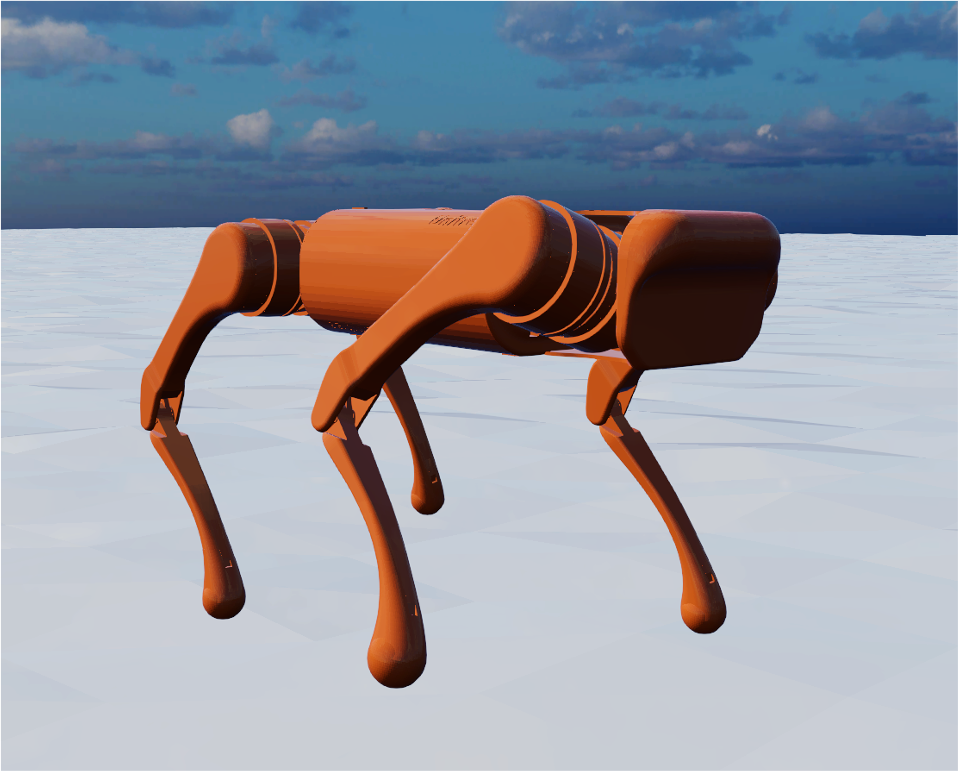
\includegraphics[width=1\linewidth]{unitree_a1.png}
\column{0.5\linewidth}
\begin{itemize}
    \item ``Движение вперед / назад''
	\item ``Движение вперед с заданной скоростью''
    \item ``Поворот по / против часовой стрелке''
\end{itemize}
\end{columns}
\textbf{Пространство наблюдений} положение корпуса, суставов, линейные и угловые скорости ($\mathcal{R}^{50}$) 
\\
\textbf{Пространство действий} целевые положения суставов ($\mathcal{R}^{12}$ )

\end{frame}

\begin{frame}{Метод обучения стратегии для управления движением
шагающего робота с заданной линейной и угловой скоростью}
\begin{multline*}
    r = k_{torso\ height} \cdot r_{torso\ height} +
    k_{torque} \cdot r_{torque} +\\
    k_{joint\ speed} \cdot r_{joint\ speed} +
    k_{slip} \cdot r_{slip} +\\
    k_{work} \cdot r_{work} + 
    k_{ground\ impact} \cdot r_{ground\ impact} +\\
    k_{z\ acceleration} \cdot r_{z\ acceleration} +  k_{velocity} \cdot r_{velocity} +\\
    k_{transverse\ and\ rotation} \cdot r_{transverse\ and\ rotation}
\label{eq:unitree_reward}
\end{multline*}

\begin{align*}
& r_{velocity} = \mathrm{clip}(V_x \cdot D / \hat{V_x}, 0, 1) \hspace{18pt}\text{``Движение вперед / назад''}\\
& r_{velocity} = \max(1 - |V_x / \hat{V_x} - 1|, 0) \hspace{1pt}\text{``Движение вперед с заданной скоростью''}\\
& r_{velocity} = \mathrm{clip}(W_z \cdot D / \hat{W_z}, 0, 1) \hspace{13pt}\text{``Поворот по / против часовой стрелки''}
\end{align*}
\end{frame}

\begin{frame}{Оценка результатов работы в симуляции}
\begin{figure}[h]
\begin{subfigure}{.5\textwidth}
  \centering
  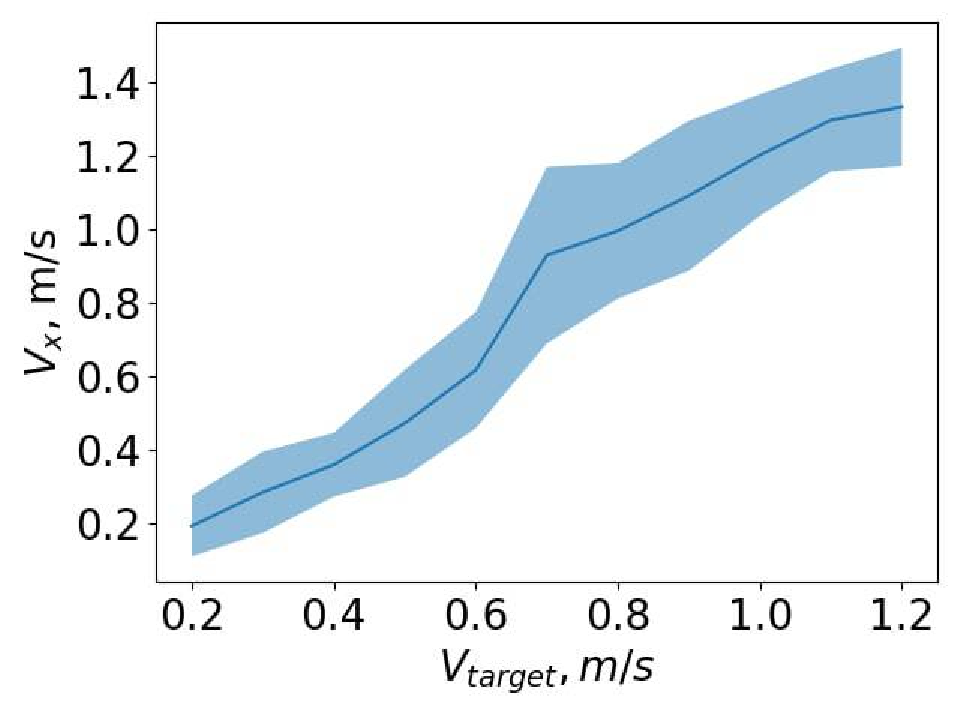
\includegraphics[width=1\textwidth]{images/vx}
\end{subfigure}%
\begin{subfigure}{.5\textwidth}
  \centering
  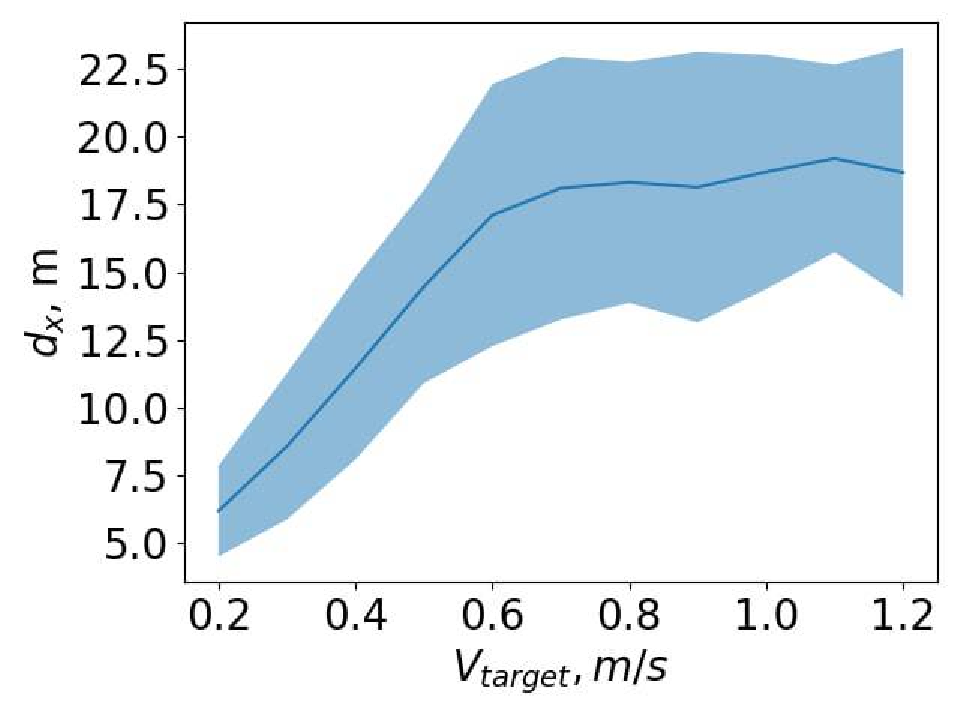
\includegraphics[width=1\textwidth]{images/dx}
\end{subfigure}%
\end{figure}
\begin{table} [htbp]
    \centering
    \begin{threeparttable}
        \begin{tabular}{| p{1cm} || p{2cm} | p{2cm} | p{2cm} |p{2cm} |}
            \hline
            \hline
            Задача & Вперед & Назад & По часовой & Против часовой \\
            \hline
            $R_{total}$ &	529 $\pm$ 124 &	508 $\pm$ 98 &	85 $\pm$ 219 &	165 $\pm$ 155 \\
            $N_{steps}$ & 3263 $\pm$ 633 &	3136 $\pm$ 545 &	2057 $\pm$ 1208 &	2095 $\pm$ 1325 \\
            \hline
            \hline
        \end{tabular}
    \end{threeparttable}
\end{table}
\end{frame}

\begin{frame}{Результаты задачи 2}
\begin{itemize}
    \item[\textcolor{ForestGreen}{\checkmark}] Был разработан метод обучения робота Unitree A1 решать различные задачи перемещения.
    \item[\textcolor{ForestGreen}{\checkmark}] Разработанная функция награды побуждает агента следовать плавной и безопасной стратегии.
\end{itemize}
\end{frame}



\section{Глава 4. Иерархический алгоритм, комбинирующий алгоритмический и
нейросетевой подходы и его применение для управления агентом в среде NetHack}

\begin{frame}
    \frametitle{Задачи исследования}
    \begin{itemize} 
        \item \underline{Задача 1.} Разработка метода, способного оперировать действиями различного масштаба, устойчивого к шумам, и его применение для настройки оптического интерферометра (вызов 1,2).
        \item \underline{Задача 2.} Разработка метода, который позволяет достичь сходимости к хорошему оптимуму для многозадачного агента и его применение  для управления движением шагающего робота (вызов 3).
        {\color{orange}\item \underline{Задача 3.} Разработка иерархического алгоритма, который комбинирует алгоритмический и нейросетевой подходы и его применение для управления агентом в среде NetHack (вызов 4).}
    \end{itemize}
\end{frame}

\begin{frame}{Постановка задачи оптимизации}

$$V(s_t) = \max_{a \in \mathcal{A}}\ex_{r_{t+1},s_{t+1}}\left[r_{t+1} + \gamma V(s_{t+1})\right]$$
$$\pi(s_t) = \argmax_{a \in \mathcal{A}}\ex_{r_{t+1},s_{t+1}}\left[r_{t+1} + \gamma V(s_{t+1})\right]$$

Особенности:
\begin{enumerate}
    \item Процедурная генерация среды.
    \item Разреженная функция награды $|s| \ll |\mathcal{S}|: r(s,a,s') \neq 0$.
    \item Необходимость следования различным стратегиям в зависимости от текущего состояния. 
    \item Многомодальные наблюдения $s = (s_{\mathrm{text}}, s_{\mathrm{img}}, s_{\mathrm{num}})$.
\end{enumerate}
\end{frame}

\setcounter{footnote}{0} 
\begin{frame}{Алгоритм: объединение обучаемых и алгоритмических стратегий в иерархического агента\footnotemark[1,2]}

\begin{minipage}{\linewidth}
\begin{columns}
\column{0.5\linewidth}
\begin{enumerate}
    \item Декомпозиция на отдельные стратегии может существенно помочь в задачах, где нужно уметь переключаться между различными навыками.
    \item Переключение между обучаемыми и алгоритмическими стратегиями происходит в зависимости от состояния среды. 
\end{enumerate}

\column{0.5\linewidth}
\begin{algorithm}[H]
\SetKwComment{Comment}{/* }{ */}
\SetKw{Continue}{continue}
\KwData{condition, $\pi_{\theta}$, $<\pi_{\mathrm{alg}}>$}
\While{not done}{
  \eIf{condition($s_t$)}{
    $a_t \sim \pi_{\theta}(s_t)$\;
  }{
    $\pi = \mathrm{rank}(\pi_{\mathrm{alg}}, s_t)$\;
    $a_t \sim \pi(s_t)$\;
  }
  $s_{t+1} \sim p(s_{t+1}|s_t,a_t)$\;
}
\end{algorithm}
\end{columns}
\end{minipage}

\begin{minipage}{\linewidth}

%\footnote[frame]{Sutton, R., et.all. Between MDPs and semi-MDPs: A framework for temporal abstraction in reinforcement learning. Artificial Intelligence (1999)}
\end{minipage}
\footnotetext[1]{Barreto, A., et al., The Option Keyboard: Combining Skills in Reinforcement Learning, NeurIPS, 2019.}
\footnotetext[2]{Gao, J., et al., Deep Reinforcement Learning for Indoor Mobile Robot Path Planning, Sensors (Basel), 2020.}
    
\end{frame}

\begin{frame}
\frametitle{Задача: NetHack challenge}
\begin{columns}
\column{0.6\linewidth}
  \centering
  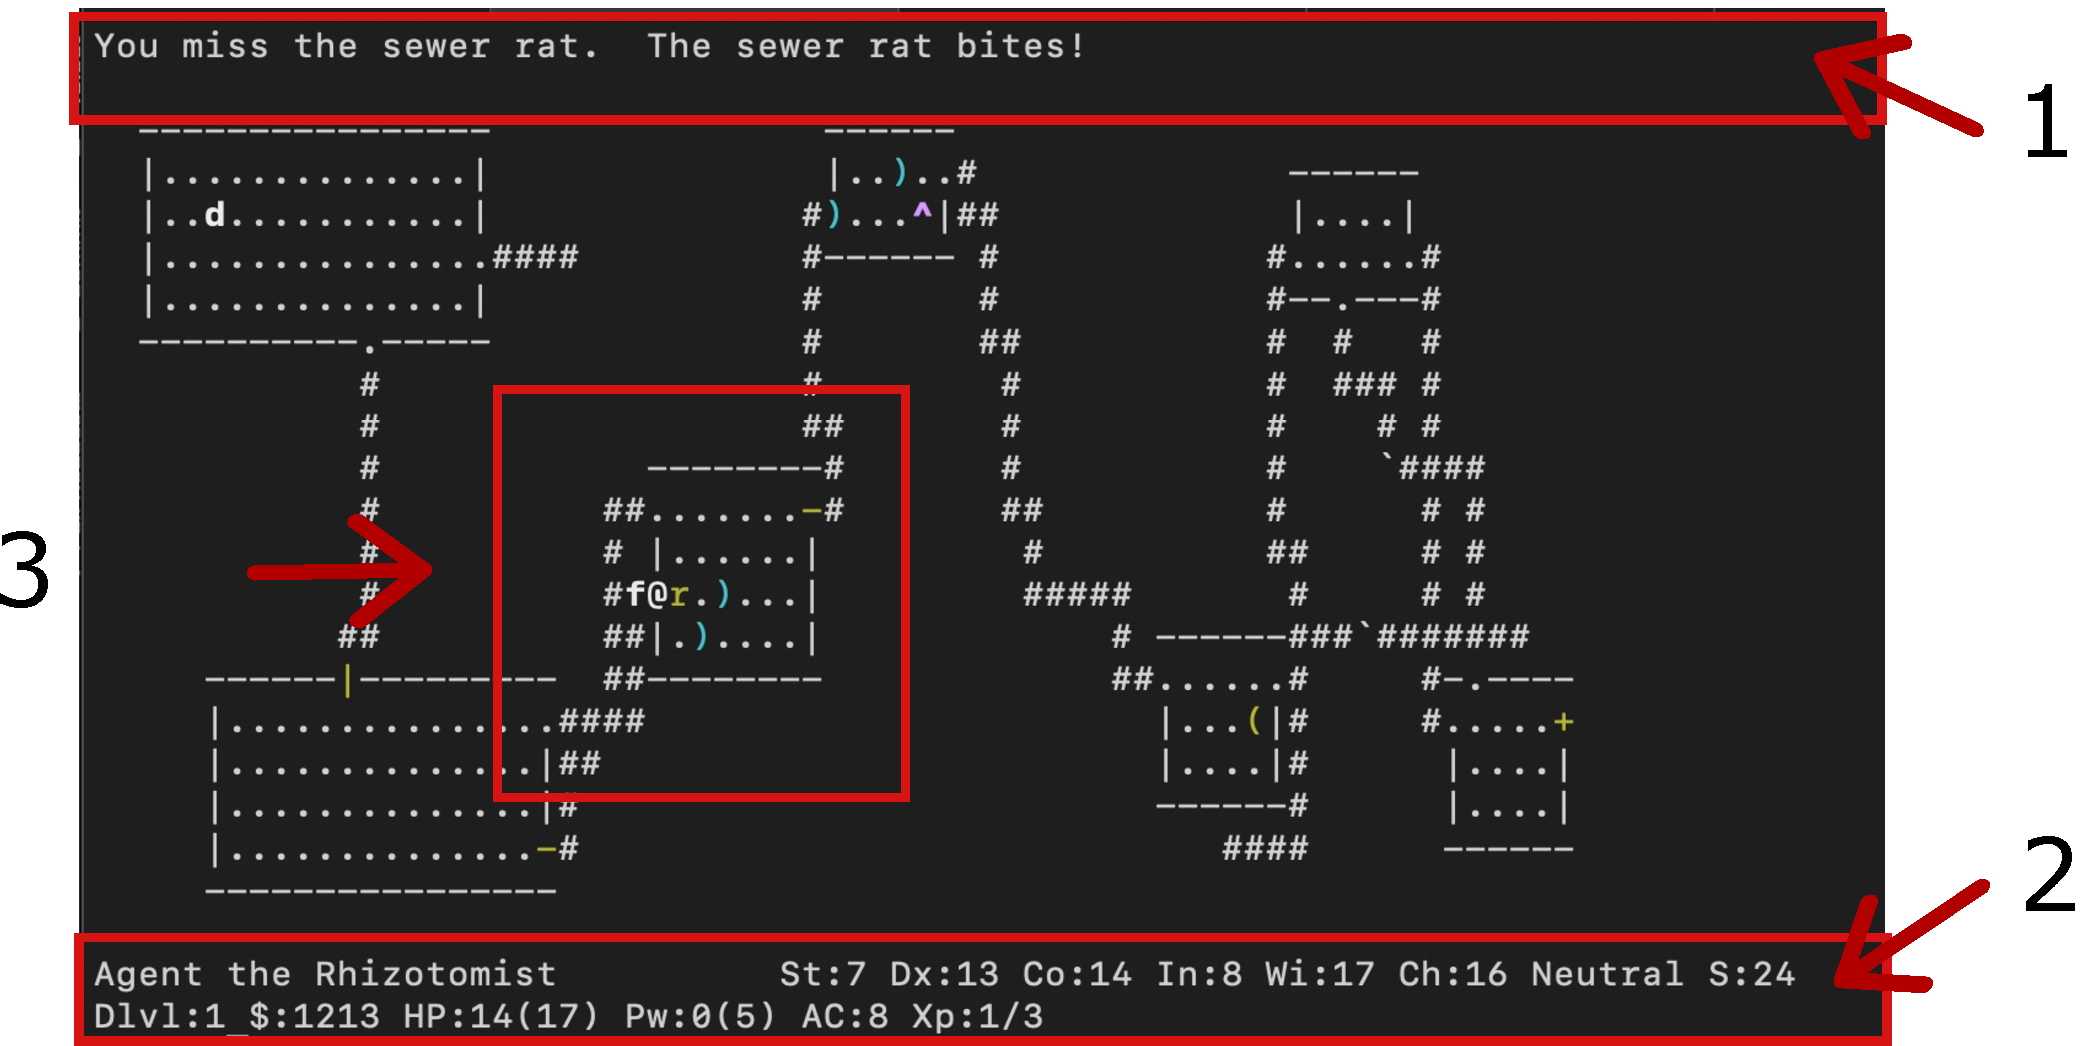
\includegraphics[width=1\linewidth]{images/nethack_map_view.pdf}
\column{0.55\linewidth}
\begin{enumerate}
    \item текстовое сообщение описывающее текущее событие
    \item статистика агента (здоровье, золото, сила, и др.) 
    \item окно центрированное возле текущего положения агента (@).
\end{enumerate}
\end{columns} 
\vspace{20pt}
В чем ``challange''?
\begin{itemize}
    \item Процедурная генерация среды
    \item NetHack – очень длинная игра
    \item Много модальные наблюдения
    \item Сложное пространство действий
\end{itemize}


\end{frame}

\subsection{Декомпозиция игры NetHack на подзадачи}

\begin{frame}{Декомпозиция игры NetHack на подзадачи}
\begin{columns}
\column{0.5\linewidth}
\centering
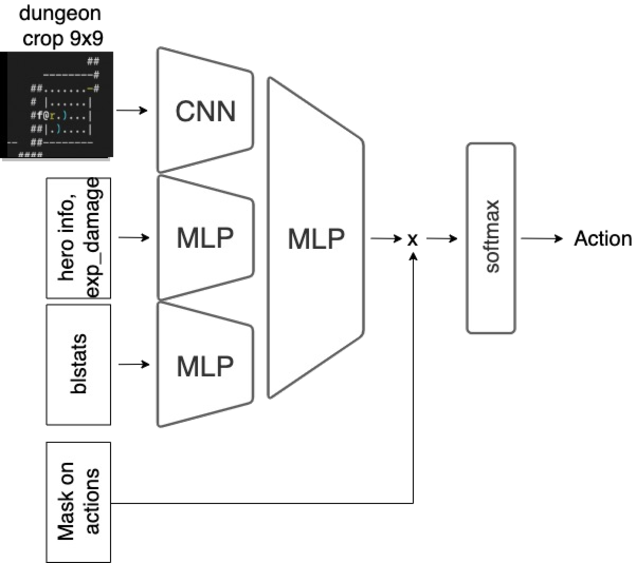
\includegraphics[width=1\linewidth]{images/raph_arch.pdf}
\column{0.5\linewidth}
\textbf{Пространство действий}. 
\begin{itemize}
    \item шаг или ближняя атака (x8 направлений)
    \item дальняя атака (x8 направлений)
    \item пропуск хода
    \item заклинание Elbereth
    \item молитва
\end{itemize}
\textbf{Передача управления}. 
$distance(agent, monster) < 5$
\end{columns}
\end{frame}

\subsection{Объединение RL и алгоритмического подхода}

\begin{frame}
\frametitle{Обучение иерархического агента совмещающего обучение с подкреплением и алгоритмический подход}
\begin{columns}
\column{0.7\linewidth}
\centering
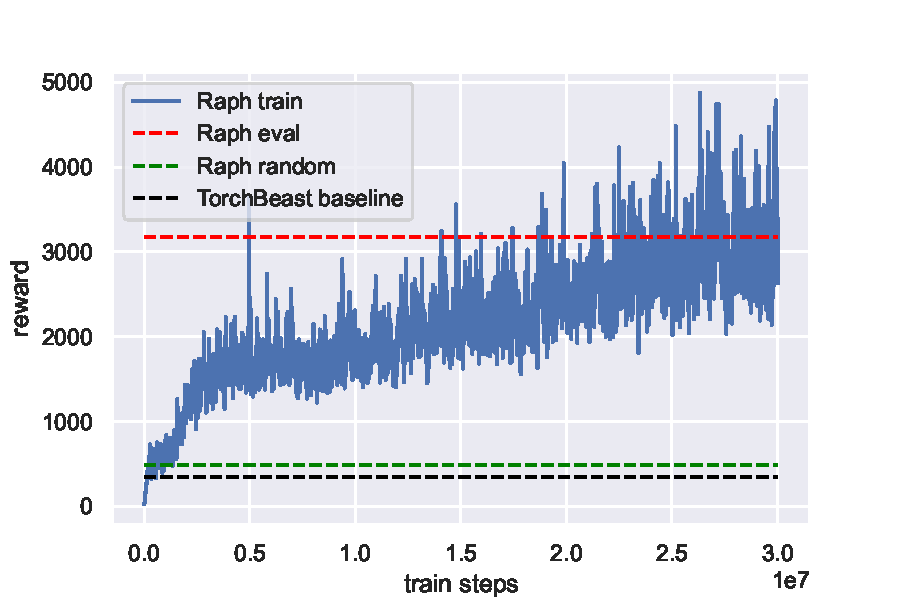
\includegraphics[width=1\linewidth]{images/raph_train.pdf}
\column{0.5\linewidth}
\begin{itemize}
    \item ближняя атака 66\%
    \item дальняя атака 21.6\%
    \item пропуск хода 11\%
    \item ``Elbereth'' 0.3\%
    \item молитва 0.1\%
\end{itemize}
\end{columns}
\end{frame}


\begin{frame}{Результаты задачи 3}
\begin{itemize}
    \item[\textcolor{ForestGreen}{\checkmark}] Предложен метод объединения обучаемого и алгоритмического подходов в рамках одного агента. С использованием предложенного метода реализован гибридный нейро-символьный агент для среды NetHack.
    \item[\textcolor{ForestGreen}{\checkmark}] В реализованном методе RL агент решает одну из наиболее сложных задач возникающих в среде NetHack — сражение с монстрами.
    \item[\textcolor{ForestGreen}{\checkmark}] В соревновании по игре NetHack (NeurIPS 2021 Competition Track) агент занял \textcolor{orange}{первое место} среди 37 команд из 19 стран мира.
\end{itemize}
    
\end{frame}

%\begin{frame}
%    \frametitle{Изображения по-вертикали}
%    \centering
%    \vfill
%    \includegraphics[width=0.8\linewidth,height=0.1\textheight]{latex%} \\
%    \TeX
%    \vfill
%    \includegraphics[width=0.8\linewidth,height=0.2\textheight]{latex%} \\
%    \LaTeX
%    \vfill
%    \includegraphics[scale=0.2]{latex} \\
%    \vfill
%\end{frame}


%\begin{frame}
%    \frametitle{Изображения по-горизонтали}
%    \begin{minipage}[t]{0.47\linewidth}
%        \textbf{Составная \\ подпись 1}
%        \center{\includegraphics[width=1\linewidth]{knuth1}}
%    \end{minipage}
%    \hfill
%    \begin{minipage}[t]{0.47\linewidth}
%        \textbf{Составная \\ подпись 2}
%        \center{\includegraphics[width=1\linewidth]{knuth2}}
%    \end{minipage}
%\end{frame}


%\begin{frame}
%    \frametitle{Разделяющие линии}
%    \begin{minipage}[c]{0.47\linewidth}
%        \center{\includegraphics[width=1\linewidth]{latex}}
%        \bigskip
%        \hrule{}
%        \bigskip
%        \textbf{Составная \\ подпись 1}
%    \end{minipage}
%    \hfill
%    \vrule{}
%    \hfill
%    \begin{minipage}[c]{0.47\linewidth}
%        \flushright
%        \textbf{Составная \\ подпись 2}
%        \center{\includegraphics[width=1\linewidth]{knuth2}}
%    \end{minipage}
%\end{frame}

%\begin{frame}
%    \frametitle{Четыре изображения}
%    \centering
%    \includegraphics[width=0.35\linewidth,angle=35]{latex}
%    \includegraphics[width=0.35\linewidth,angle=135]{latex}\\
%    \includegraphics[width=0.35\linewidth,angle=15]{latex}
%    \includegraphics[width=0.35\linewidth,angle=-15]{latex}
%\end{frame}

       % Настройки заглавной странице
\begin{frame}
    \frametitle{Научная новизна}
    \begin{itemize}
        \item Впервые реализован \dots
        \item Разработана программа \dots
        \item Впервые проведён анализ \dots
        \item Предложена схема \dots
    \end{itemize}
\end{frame}
\note{
    Проговаривается вслух научная новизна
}

\begin{frame}
    \frametitle{Научная и практическая значимость}
    \begin{itemize}
        \item Получены выражения для \dots.
        \item Определены условия \dots.
        \item Разработаны устройства \dots.
    \end{itemize}
\end{frame}
\note{
    Проговариваются вслух научная и практическая значимость
}

\begin{frame}
    \frametitle{Свидетельство о регистрации программы}
    \begin{figure}[h]
        \centering
        \includegraphics[height=0.7\textheight]{registration}
    \end{figure}
\end{frame}
\note{
    Получено свидетельство о регистрации разработанной программы \textsc{Hello~world™}.
}

\begin{frame}
    \frametitle{Акт о внедрении}
    \begin{figure}[h]
        \centering
        \fbox{
            \begin{minipage}[t]{0.4\linewidth}
                \includegraphics[width=\linewidth]{implementation}
            \end{minipage}
        }
    \end{figure}
\end{frame}
\note{
    Получен акт о внедрении.
}

\begin{frame} % публикации на одной странице
% \begin{frame}[t,allowframebreaks] % публикации на нескольких страницах
    \frametitle{Основные публикации}
    \nocite{vakbib1}%
    \nocite{vakbib2}%
    %
    %% authorwos
    \nocite{wosbib1}%
    %
    %% authorscopus
    \nocite{scbib1}%
    %
    %% authorconf
    \nocite{confbib1}%
    \nocite{confbib2}%
    \nocite{confbib3}%
    %
    %% authorother
    \nocite{bib1}%
    \nocite{bib2}%
    \ifnumequal{\value{bibliosel}}{0}{
        \insertbiblioauthor
    }{
        \printbibliography%
    }
\end{frame}
\note{
    Результаты работы опубликованы в N печатных изданиях,
    в~т.\:ч. M реферируемых изданиях.
}

\begin{frame}
    \frametitle{Участие в конференциях}
    \begin{itemize}
        \item Научная сессия МГУ, Москва 2013--2015;
        \item \rom{24} Russian Conference (RuC 2014), Obninsk, Russia, 2014
        \item \rom{7} International Conference (IAC 16), Busan, Korea,
              2016;
        \item \rom{28} Other Conference (AC 16), East Lansing, MI USA, 2016;
        \item \dots
    \end{itemize}
\end{frame}
\note{
    Работа была представлена на ряде конференций.
}

\begin{frame}[plain, noframenumbering] % последний слайд без оформления
    \begin{center}
        \Huge
        Спасибо за внимание!
    \end{center}
\end{frame}
    % Последние слайды презентации
\appendix
\begin{frame}
\frametitle{Математическая модель интерферометра Маха-Цендера без линз}
\begin{columns}
\column{0.6\linewidth}
  \centering
  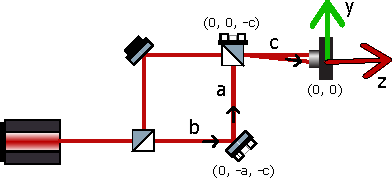
\includegraphics[width=1\linewidth]{images/MZI_matmodel.pdf}
  \begin{itemize}
    \item управление положением луча на камере $(x_0, y_0)$
    \item управление направлением $\vec{k}$
  \end{itemize}

\column{0.5\linewidth}
\begin{table} [htbp]
    \centering
    \begin{threeparttable}
        \begin{tabular}{| p{2.5cm} || p{2cm} |}
            \hline
            \hline
            параметр & значение \\
            \hline
            Mirror 2 $\to$ BS 2 & 200 mm\\
            BS 1 $\to$ Mirror 2 & 300 mm\\
            BS 2 $\to$ Camera & 100 mm\\
            radius & 0.95\\
            $\alpha_{{\mathrm{max}}(x,1)}$ & $5.2 \cdot 10^{-3}$ rad\\
            $\alpha_{{\mathrm{max}}(y,1)}$ & $3.7 \cdot 10^{-3}$ rad\\
            $\alpha_{{\mathrm{max}}(x,2)}$ & $2.6 \cdot 10^{-3}$ rad\\
            $\alpha_{{\mathrm{max}}(y,2)}$ & $1.8 \cdot 10^{-3}$ rad\\
            \hline
            \hline
        \end{tabular}
    \end{threeparttable}
\end{table}

\end{columns} 
\end{frame}


\begin{frame}
\frametitle{Примеры интерференционных картин без линз полученные в симуляции}
\begin{columns}
\column{0.7\linewidth}
  \centering
   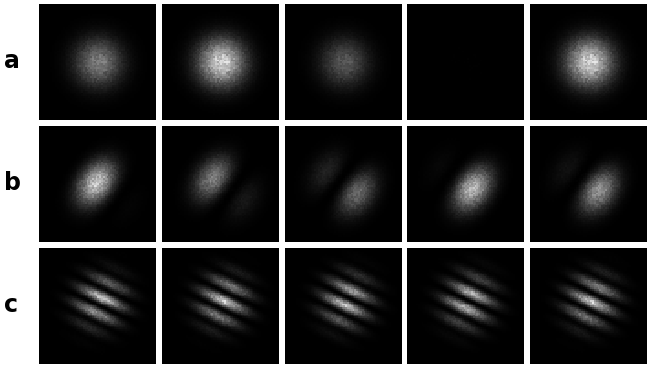
\includegraphics[scale=0.4]{images/visib_expl.png}

\column{0.5\linewidth}
\begin{description}
    \item V = 1
    \vspace{30pt}
    \item V = 0.3
    \vspace{30pt}
    \item V = 0.0026
\end{description}

\end{columns} 
\end{frame}


\begin{frame}
\frametitle{Математическая модель интерферометра Маха-Цендера с линзами}
\begin{columns}
\column{0.6\linewidth}
  \centering
   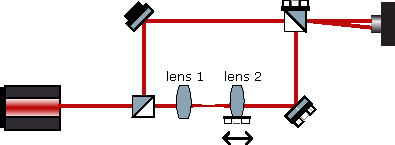
\includegraphics[width=1\linewidth]{images/MZI_expl_lenses.pdf}
  \begin{itemize}
    \item управление положением луча на камере $(x_0, y_0)$
    \item управление направлением $\vec{k}$
    \item \textcolor{red}{управление волновым фронтом}
  \end{itemize}

\column{0.5\linewidth}
\begin{table} [htbp]
    \centering
    \begin{threeparttable}
        \begin{tabular}{| p{2.5cm} || p{2cm} |}
            \hline
            \hline
            параметр & значение \\
            \hline
            BS 1 $\to$ Lens 1 & 50 mm\\
            $f_{\mathrm{lens 1}}$ = $f_{\mathrm{lens 2}}$ & 50 mm\\
            radius & 0.71 mm\\
            $\Delta_{\mathrm{max}}$ & 4.2 mm\\
            \hline
            \hline
        \end{tabular}
    \end{threeparttable}
\end{table}

\end{columns} 
\end{frame}

\begin{frame}
    \frametitle{Примеры интерференционных картин полученные на интерферометре Маха-Цендера с линзами}
    \centering
    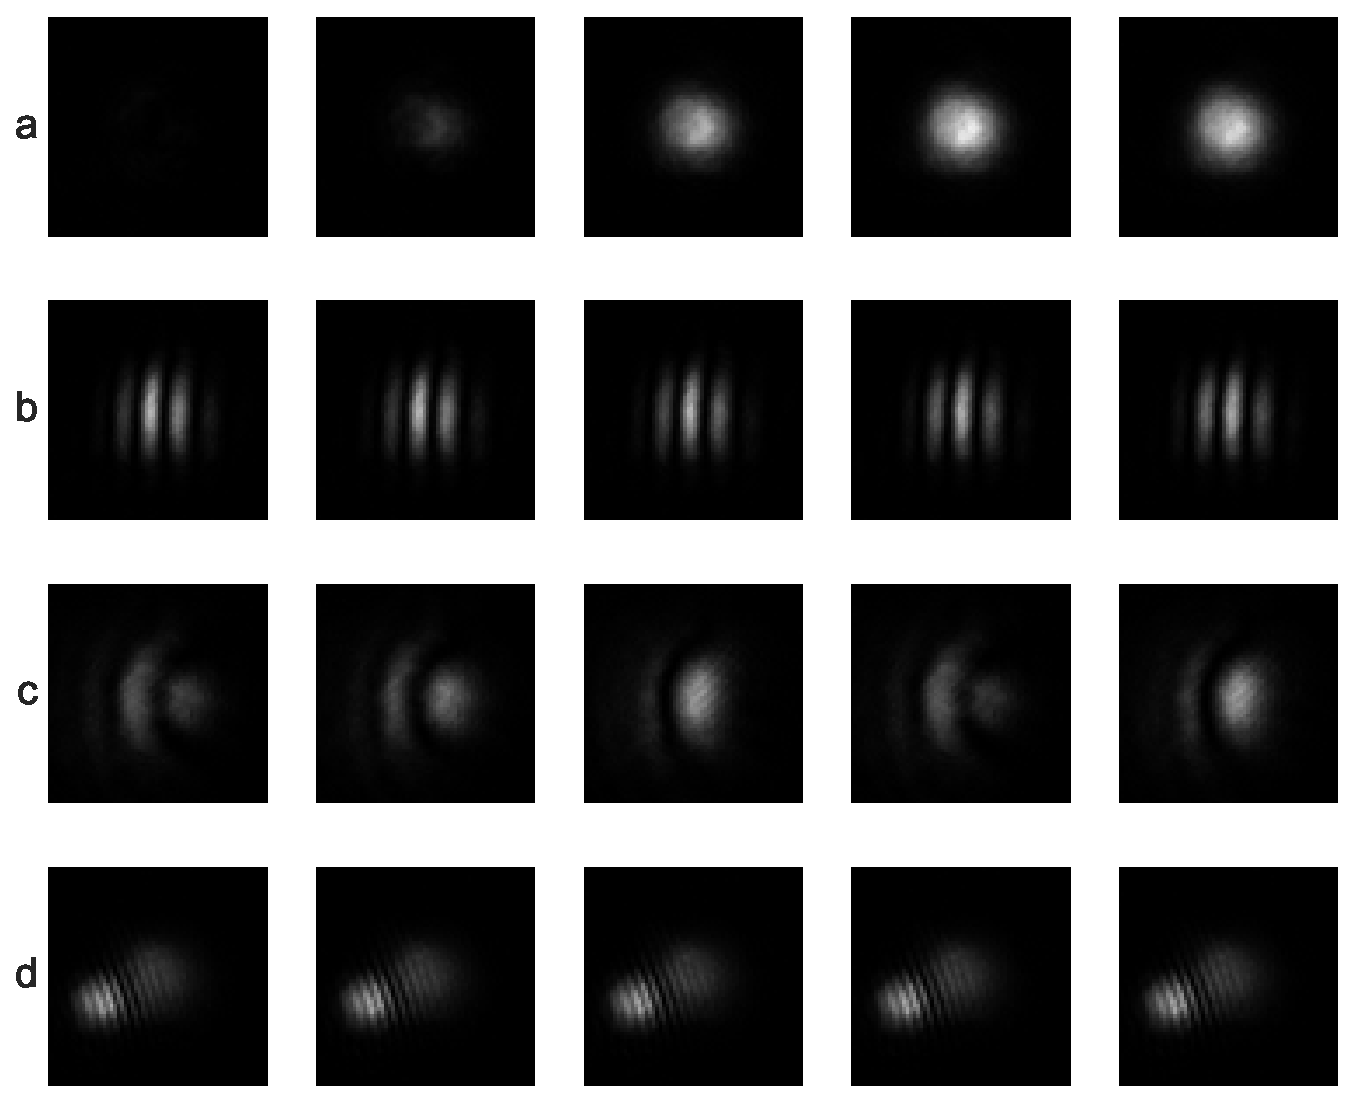
\includegraphics[width=0.8\linewidth]{images/Env_patterns.pdf}
\end{frame}

\begin{frame}
\frametitle{Видность интерференционной картины в интерферометре
Маха-Цендера без линз}

\begin{columns}
\column{0.4\linewidth}
\centering
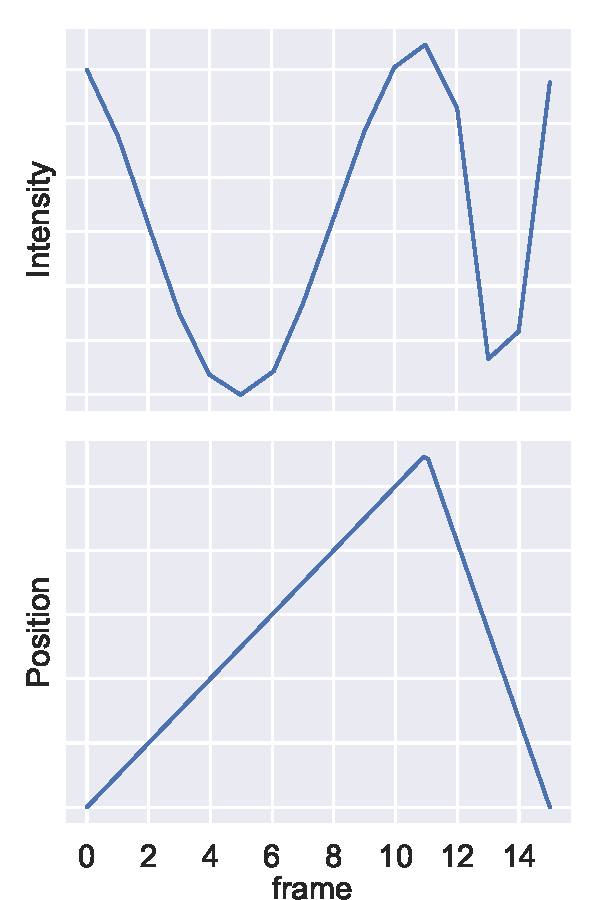
\includegraphics[width=1\linewidth]{piezo.pdf}

\column{0.5\linewidth}
\begin{align*}
& I(x,y,t)=|E_1(x,y,0)+E_2(x,y,0)e^{i\phi_{\mathrm{piezo}}(t)}|^2 \\
& I_{\mathrm{tot}}(t) = \iint_{-\infty}^{+\infty} I(x, y, t) {\mathrm{d}}x{\mathrm{d}}y \\
& V = \frac{            
        \max_{t}(I_{\mathrm{tot}}) - \min_t(I_{\mathrm{tot}})}
        {\max_{t}(I_{\mathrm{tot}}) + \min_t(I_{\mathrm{tot}})} \\
& V = \exp\left(- \frac{x_0^2 + y_0^2}{2 r^2}\right)  \exp\left[- \frac{(k_x^2 + k_y^2) r^2}{8}\right] \\
\end{align*}

\end{columns}
\end{frame}

\begin{frame}
\frametitle{Видность интерференционной картины в интерферометре Маха-Цендера с линзами}
\begin{columns}
\column{0.3\linewidth}
\begin{align*}
& \dfrac{1}{q} = \dfrac{1}{\rho} - \dfrac{i \lambda}{\pi r^2} \\
& q^{\prime}=\dfrac{A q+B}{C q+D}\\
\end{align*}
\column{0.7\linewidth}
\begin{align*}
& \begin{bmatrix} A & B \\ C & D \end{bmatrix}=\begin{bmatrix} 1 & d \\ 0 & 1 \end{bmatrix} \hspace{25pt}\text{вакуум длины $d$}\\
& \begin{bmatrix} A & B \\ C & D \end{bmatrix}=\begin{bmatrix} 1 & 0 \\ -1/f & 1 \end{bmatrix} \hspace{5pt}\text{линза с фокусным расстоянием $f$} \\
& M = M_3^{ABCD} \times M_2^{ABCD} \times M_1^{ABCD}
\end{align*}
\end{columns}

\begin{equation*}
\begin{split}
    V =\frac{4}{\left(n^{2}+1\right) r_{\mathrm{u}}^{2}} \frac{1}{c} \exp \left(-\left(x_{0}^{2}+y_{0}^{2}\right)\left(\frac{1}{r_{\mathrm{u}}^{2} n^{2}}-\frac{n^{2}+1}{n^{6} r_{\mathrm{u}}^{6} c^{2}}\right)\right) \times \\ \times \exp \left(-\frac{n^{2}+1}{4 c^{2} n^{2} r_{\mathrm{u}}^{2}}\left(k_{x}^{2}+k_{y}^{2}\right)\right) \exp \left(\frac{\frac{\pi}{\lambda \rho^{\prime}}}{n^{2} r_{\mathrm{u}}^{2} c^{2}}\left(x_{0} k_{x}+y_{0} k_{y}\right)\right),
\end{split}
\end{equation*}
параметр $n=\dfrac{r_{\mathrm{l}}}{r_{\mathrm{u}}}$, $c^2 = (\dfrac{n^2 + 1}{n^2r^2_{\mathrm{u}}})^2$
\end{frame}

\begin{frame}{Анализ стратегии дискретного DQN агента}

\begin{minipage}{\textwidth}
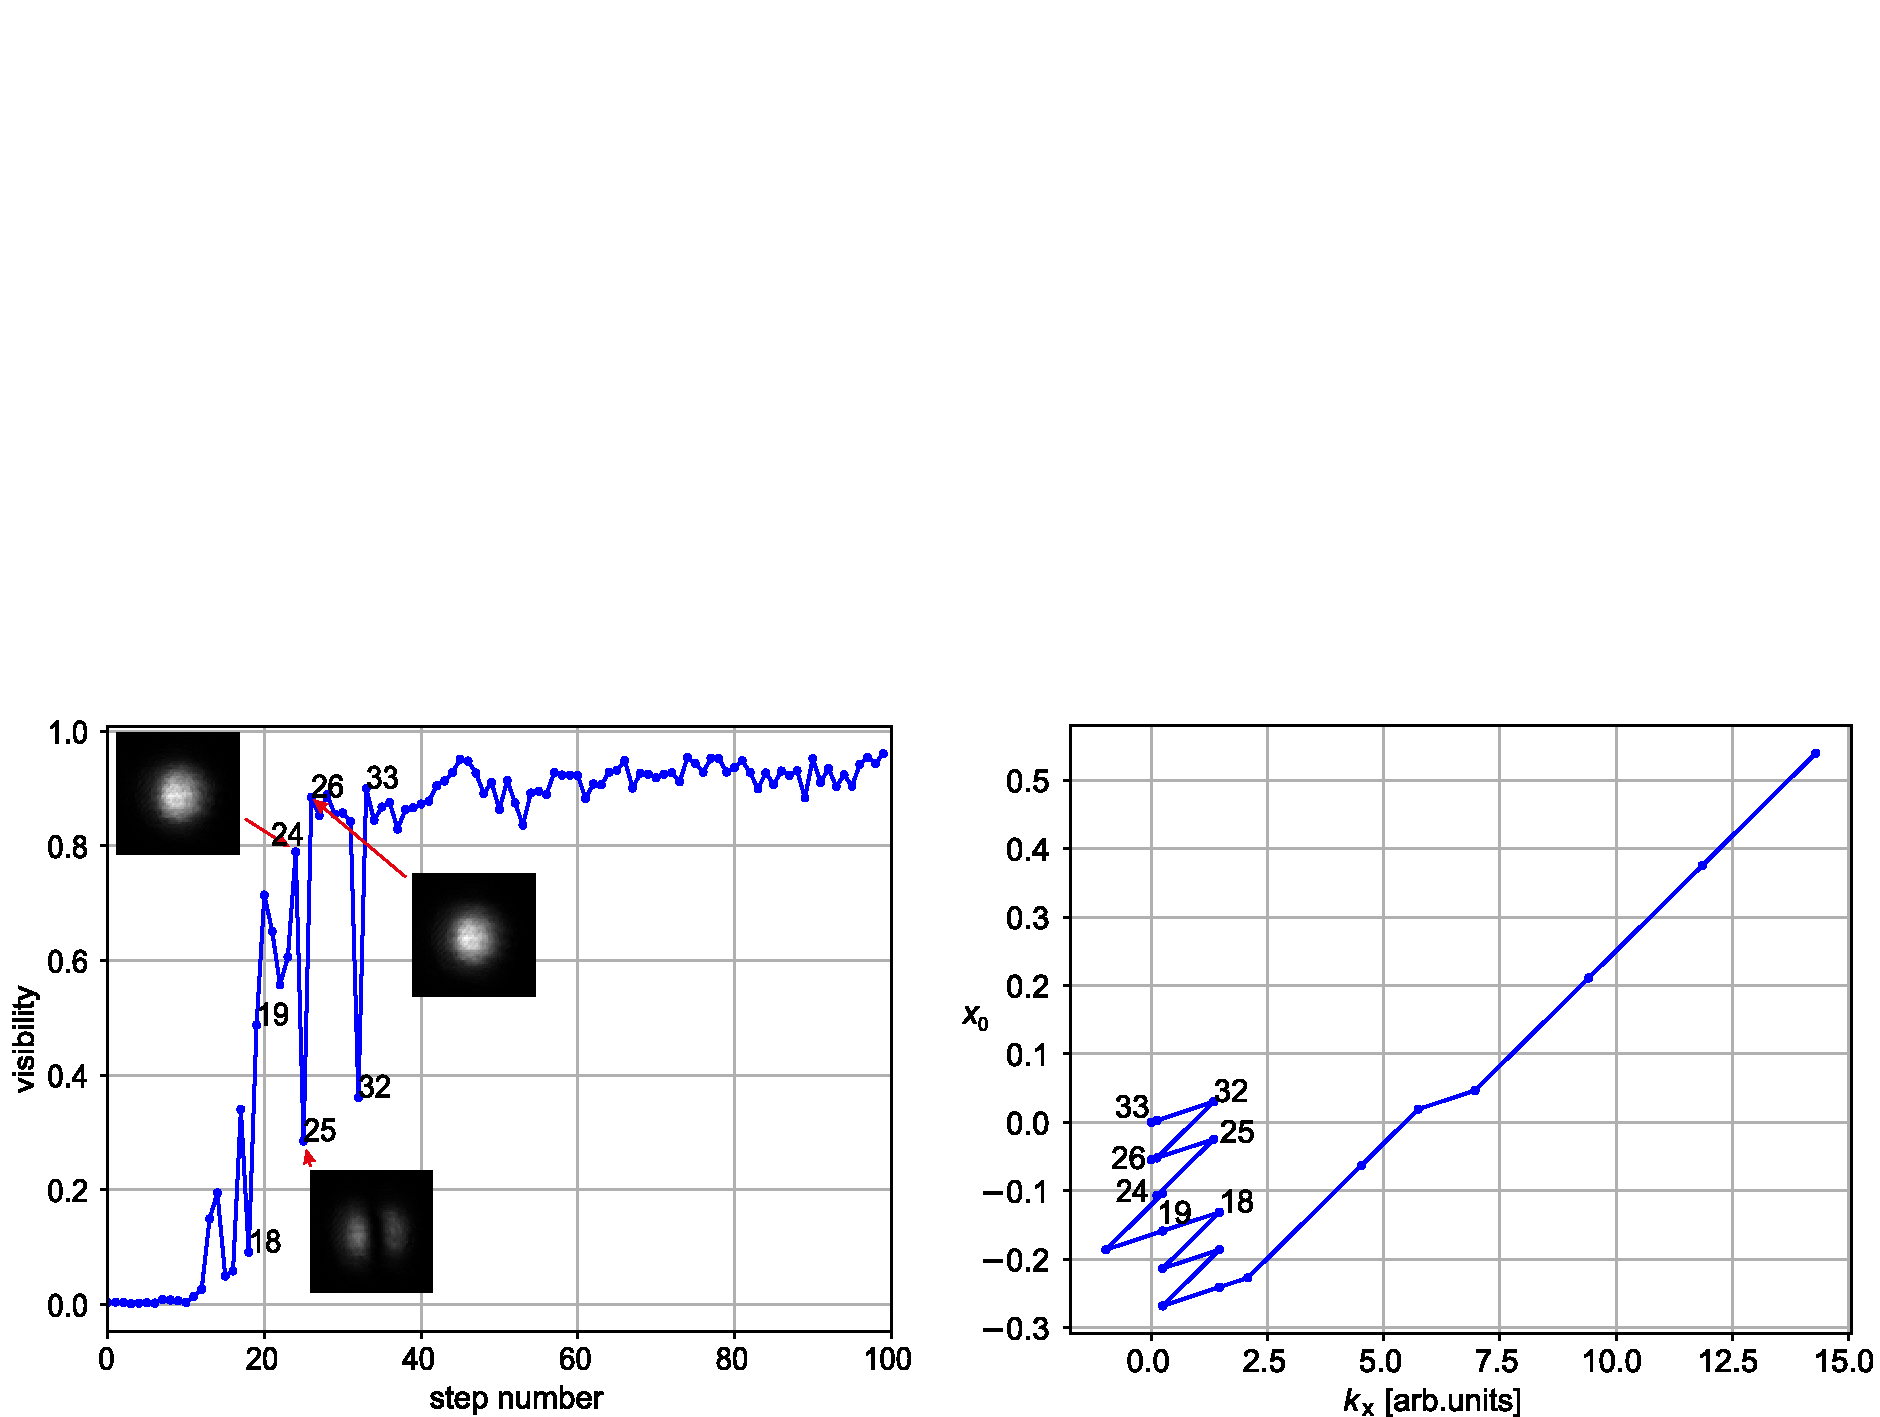
\includegraphics[width=1\linewidth]{DQN_analysis.pdf}
\end{minipage}
\begin{minipage}{\textwidth}
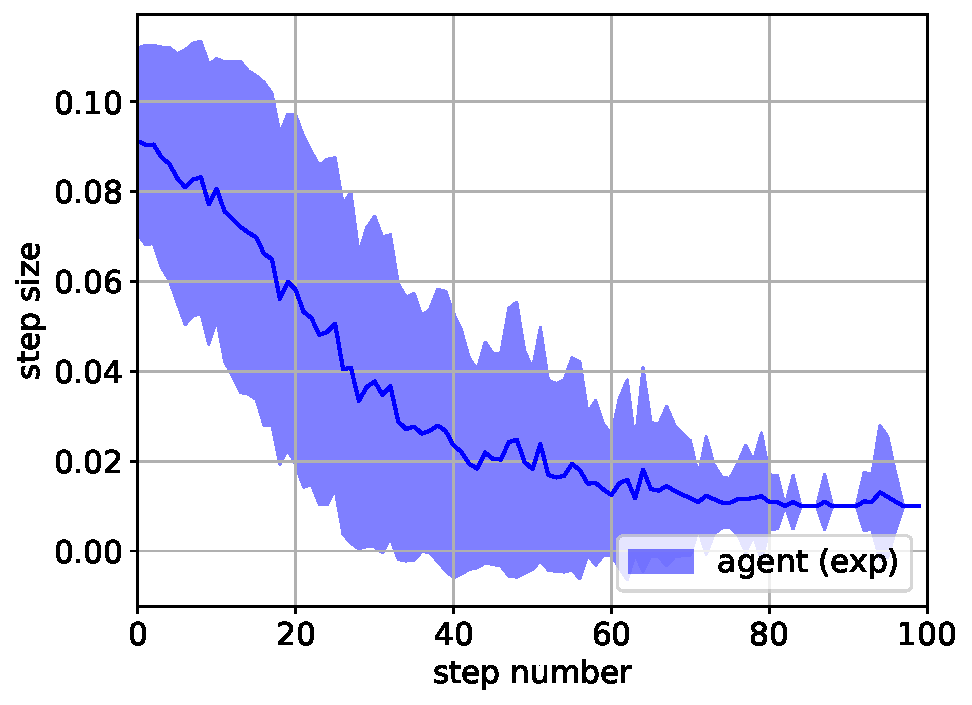
\includegraphics[width=0.5\linewidth]{images/agent_step_size.pdf}
\end{minipage}
\end{frame}

\begin{frame}{Анализ стратегии непрерывного TD3 агента}
\begin{columns}
\column{0.5\linewidth}
\centering
\includegraphics[width=1\linewidth]{Presentation/images/parallel_actions.png}
Процент "параллельных действий"
\column{0.5\linewidth}
\centering
\includegraphics[width=1\linewidth]{Presentation/images/action_norm_decrease.png}
Средняя амплитуда действий
\end{columns}
\end{frame}

\begin{frame}{Репортаж 1 канала}
    
\end{frame}


%\begin{frame}
%    \frametitle{Ответы на замечания ведущей организации %НИИ~<<Рога~и~копыта>>}
%    \begin{itemize}
%        \item Замечание -- ответ
%        \item Замечание -- ответ
%        \item Замечание -- ответ
%        \item Замечание -- ответ
%        \item Замечание -- ответ
%    \end{itemize}
%\end{frame}

%\begin{frame}
%    \frametitle{Ответы на замечания оф. оппонента %Иванова\,И.\,И}
%    \begin{itemize}
%        \item Замечание -- ответ
%        \item Замечание -- ответ
%        \item Замечание -- ответ
%        \item Замечание -- ответ
%        \item Замечание -- ответ
%    \end{itemize}
%\end{frame}

%\begin{frame}
%    \frametitle{Ответы на замечания Петрова\,П.\,П}
%    \begin{itemize}
%        \item Замечание -- ответ
%        \item Замечание -- ответ
%        \item Замечание -- ответ
%        \item Замечание -- ответ
%        \item Замечание -- ответ
%    \end{itemize}
%\end{frame}
      % Запасные слайды презентации
\end{document}
